\documentclass[aspectratio=169,11pt]{beamer}
\usetheme{metropolis}
\usepackage{tikz}
\usetikzlibrary{arrows.meta,positioning,decorations.pathmorphing,calc,shapes.geometric,decorations.pathreplacing,patterns}
\usepackage{pgfplots}
\pgfplotsset{compat=1.18}
\usepackage{booktabs}
\usepackage{xcolor}
\usepackage{amsmath,amssymb}
\usepackage{graphicx}
\graphicspath{{figures/generated/}}
\usepackage{hyperref}
\hypersetup{colorlinks=true,urlcolor=grass,linkcolor=black,citecolor=black}
\usepackage{multirow}

\definecolor{grass}{HTML}{2E7D32}
\definecolor{circle}{HTML}{E91E63}
\definecolor{das}{HTML}{2196F3}
\definecolor{vae}{HTML}{9C27B0}
\definecolor{nldas}{HTML}{FF9800}
\definecolor{neutral}{HTML}{9E9E9E}
\definecolor{pass}{HTML}{4CAF50}
\definecolor{fail}{HTML}{F44336}
\definecolor{stoch}{HTML}{FF9800}
\definecolor{never}{HTML}{F44336}
\definecolor{always}{HTML}{4CAF50}
\definecolor{bg}{HTML}{FAFAFA}
\definecolor{memo}{HTML}{795548}

\newcommand{\Gr}{\mathrm{Gr}}
\newcommand{\IIA}{\mathrm{IIA}}
\newcommand{\R}{\mathbb{R}}
\newcommand{\Z}{\mathbb{Z}}

\title{Not All Representations Are Subspaces}
\subtitle{A Grassmannian atlas of causal structure in grokking}
\author{Elliot Tower}
\date{2026}
\institute{}

\begin{document}

\maketitle

%% --- OVERVIEW ---
\begin{frame}{Overview}
\begin{columns}[T]
\begin{column}{0.32\textwidth}
\textbf{\hyperlink{part1}{Part 1: Setup}}
\begin{enumerate}
  \item \hyperlink{sec1}{What is a causal variable?}
  \item \hyperlink{sec2}{DAS and the Grassmannian}
  \item \hyperlink{sec3}{Why linearity matters}
\end{enumerate}
\vspace{0.5em}
\textbf{\hyperlink{part2}{Part 2: The atlas}}
\begin{enumerate}
  \setcounter{enumi}{3}
  \item \hyperlink{sec4}{14 operations, three classes}
  \item \hyperlink{sec5}{Linear DAS fails completely}
  \item \hyperlink{sec6}{Stochastic grokking}
\end{enumerate}
\end{column}
\begin{column}{0.32\textwidth}
\textbf{\hyperlink{part3}{Part 3: The vacuity problem}}
\begin{enumerate}
  \setcounter{enumi}{6}
  \item \hyperlink{sec7}{Memorization artifacts}
  \item \hyperlink{sec8}{Nonlinear DAS is vacuous}
  \item \hyperlink{sec9}{Intervention faithfulness}
\end{enumerate}
\vspace{0.5em}
\textbf{\hyperlink{part4}{Part 4: The fix}}
\begin{enumerate}
  \setcounter{enumi}{9}
  \item \hyperlink{sec10}{Structured VAE}
  \item \hyperlink{sec11}{Cross-task transfer}
  \item \hyperlink{sec12}{IOI is not Grassmannian}
\end{enumerate}
\end{column}
\begin{column}{0.32\textwidth}
\textbf{Part 4 (cont.): Connections}
\begin{enumerate}
  \setcounter{enumi}{12}
  \item \hyperlink{sec12b}{Subspaces to factors}
  \item \hyperlink{sec12c}{Weight vs.\ activation space}
\end{enumerate}
\vspace{0.5em}
\textbf{\hyperlink{part5}{Part 5: Implications}}
\begin{enumerate}
  \setcounter{enumi}{14}
  \item \hyperlink{sec13}{Four-level hierarchy}
  \item \hyperlink{sec14}{Continuous metrics}
  \item \hyperlink{sec15}{Practical advice}
  \item \hyperlink{sec16}{Conclusion}
\end{enumerate}
\end{column}
\end{columns}
\end{frame}

%% ============================================================
%% PART 1: SETUP
%% ============================================================

\begin{frame}[plain]
\hypertarget{part1}{}
\vfill
\begin{center}
  \setlength{\fboxrule}{2.5pt}%
  \fcolorbox{black}{white}{\parbox{0.7\textwidth}{\centering\vspace{0.8em}
    {\Large\bfseries Part 1}\\[0.5em]
    {\large What is a causal variable, and where does DAS look?}
  \vspace{0.8em}}}
\end{center}
\vfill
\end{frame}

\begin{frame}{In this section}
\begin{columns}[T]
\begin{column}{0.48\textwidth}
\textbf{\hyperlink{sec1}{1. What is a causal variable?}}\\[0.2em]
{\small When we say a neural network ``uses'' a concept, we mean there is a direction (or subspace) in its activations that, when edited, changes the output in a predictable way.}

\vspace{0.6em}
\textbf{\hyperlink{sec2}{2. DAS and the Grassmannian}}\\[0.2em]
{\small Distributed Alignment Search (DAS) finds these subspaces. Every DAS solution is a point on a specific mathematical object: the Grassmannian manifold. This is the hidden assumption.}
\end{column}
\begin{column}{0.48\textwidth}
\textbf{\hyperlink{sec3}{3. Why linearity matters}}\\[0.2em]
{\small DAS assumes the causal variable is a linear subspace. This works for some variables but fails catastrophically for others --- and high IIA scores cannot tell you which case you are in.}
\end{column}
\end{columns}
\end{frame}

%% ============================================================
%% ALT SLIDES (from talk_slides) — compare with originals below
%% ============================================================

\hypertarget{sec1}{}
\section{1. What is a causal variable?}

%% ============================================================
%% ORIGINAL SLIDES
%% ============================================================

%% --- SLIDE: The interpretability goal (original) ---
\begin{frame}{The interpretability goal}

{\small We want to understand \emph{how} neural networks compute, not just \emph{what} they compute.}

\vspace{0.5em}

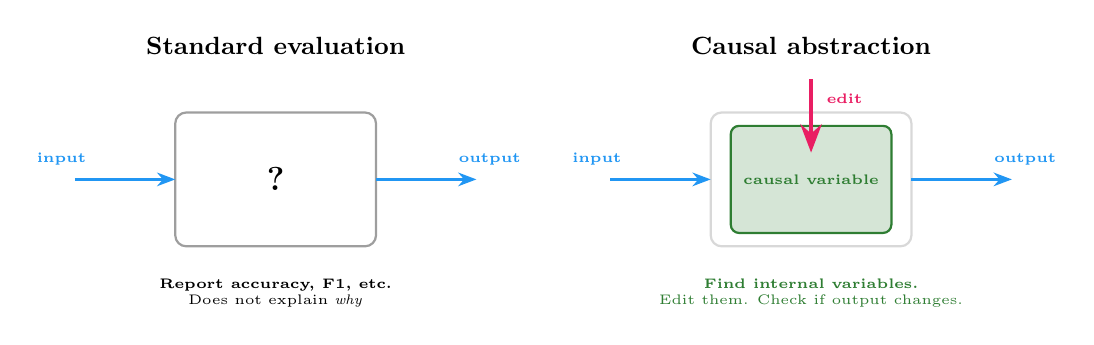
\begin{tikzpicture}[scale=0.85]
  % Left: black box
  \node[font=\small\bfseries] at (0,3.5) {Standard evaluation};
  \draw[neutral,thick,rounded corners=4pt] (-1.5,0.5) rectangle (1.5,2.5);
  \node[font=\large] at (0,1.5) {\textbf{?}};
  \draw[das,thick,-{Stealth}] (-3,1.5) -- (-1.5,1.5);
  \node[font=\tiny\bfseries,das] at (-3.2,1.8) {input};
  \draw[das,thick,-{Stealth}] (1.5,1.5) -- (3,1.5);
  \node[font=\tiny\bfseries,das] at (3.2,1.8) {output};
  \node[font=\tiny,align=center] at (0,-0.2) {\textbf{Report accuracy, F1, etc.}\\Does not explain \emph{why}};

  % Right: causal variable
  \node[font=\small\bfseries] at (8,3.5) {Causal abstraction};
  \draw[neutral!40,thick,rounded corners=4pt] (6.5,0.5) rectangle (9.5,2.5);
  \draw[das,thick,-{Stealth}] (5,1.5) -- (6.5,1.5);
  \node[font=\tiny\bfseries,das] at (4.8,1.8) {input};
  \draw[das,thick,-{Stealth}] (9.5,1.5) -- (11,1.5);
  \node[font=\tiny\bfseries,das] at (11.2,1.8) {output};

  % The causal variable inside — bigger green box, smaller text
  \fill[grass!20,rounded corners=3pt] (6.8,0.7) rectangle (9.2,2.3);
  \draw[grass,thick,rounded corners=3pt] (6.8,0.7) rectangle (9.2,2.3);
  \node[font=\tiny\bfseries,grass] at (8,1.5) {causal variable};

  % Edit arrow
  \draw[circle,ultra thick,-{Stealth}] (8,3.0) -- (8,1.9);
  \node[font=\tiny\bfseries,circle] at (8.5,2.7) {edit};

  \node[font=\tiny,grass,align=center] at (8,-0.2) {\textbf{Find internal variables.}\\Edit them. Check if output changes.};
\end{tikzpicture}

\vspace{0.3em}
{\small If editing a specific direction in the network's internal representation changes the output predictably, that direction is a \textbf{causal variable} for the behavior.}%
\footnote{\tiny Geiger et al., ``Causal Abstraction for Faithful Model Interpretation,'' 2021.}
\end{frame}

%% --- SLIDE: Interchange intervention (original) ---
\begin{frame}{Interchange intervention analysis (IIA)}

{\small The core technique: take two inputs, swap part of their internal representations, check if the output changes accordingly.}%
\footnote{\tiny Geiger et al., ``Inducing Causal Structure for Interpretable Neural Networks,'' ICML 2022.}

\vspace{0.5em}

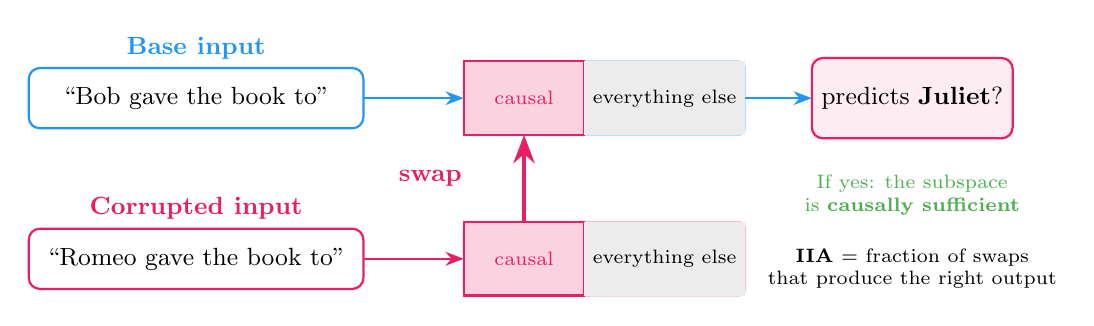
\begin{tikzpicture}[scale=0.85]
  % Base path
  \node[font=\small\bfseries,das] at (0,4.2) {Base input};
  \draw[das,thick,rounded corners=4pt] (-2.5,3.0) rectangle (2.5,3.9);
  \node[font=\small] at (0,3.45) {``Bob gave the book to''};

  % Corrupted path
  \node[font=\small\bfseries,circle] at (0,1.8) {Corrupted input};
  \draw[circle,thick,rounded corners=4pt] (-2.5,0.6) rectangle (2.5,1.5);
  \node[font=\small] at (0,1.05) {``Romeo gave the book to''};

  % Activations
  \draw[das,thick,-{Stealth}] (2.5,3.45) -- (4,3.45);
  \draw[circle,thick,-{Stealth}] (2.5,1.05) -- (4,1.05);

  % Base activation box
  \draw[das!30,thick,rounded corners=2pt] (4,2.9) rectangle (8.2,4.0);
  \fill[circle!20] (4,2.9) rectangle (5.8,4.0);
  \draw[circle,thick] (4,2.9) rectangle (5.8,4.0);
  \node[font=\scriptsize,circle] at (4.9,3.45) {causal};
  \fill[neutral!20] (5.8,2.9) rectangle (8.2,4.0);
  \node[font=\scriptsize] at (7.0,3.45) {everything else};

  % Corrupted activation box
  \draw[circle!30,thick,rounded corners=2pt] (4,0.5) rectangle (8.2,1.6);
  \fill[circle!20] (4,0.5) rectangle (5.8,1.6);
  \draw[circle,thick] (4,0.5) rectangle (5.8,1.6);
  \node[font=\scriptsize,circle] at (4.9,1.05) {causal};
  \fill[neutral!20] (5.8,0.5) rectangle (8.2,1.6);
  \node[font=\scriptsize] at (7.0,1.05) {everything else};

  % Swap arrow
  \draw[circle,ultra thick,-{Stealth}] (4.9,1.6) -- (4.9,2.9);
  \node[font=\small\bfseries,circle] at (3.5,2.25) {swap};

  % Output
  \draw[das,thick,-{Stealth}] (8.2,3.45) -- (9.2,3.45);
  \fill[circle!8] (9.2,2.85) rectangle (12.2,4.05);
  \draw[circle,thick,rounded corners=4pt] (9.2,2.85) rectangle (12.2,4.05);
  \node[font=\small,align=center] at (10.7,3.45) {predicts \textbf{Juliet}?};

  % IIA label
  \node[font=\scriptsize,pass,align=center] at (10.7,2.0) {If yes: the subspace\\is \textbf{causally sufficient}};
  \node[font=\scriptsize,align=center] at (10.7,0.9) {\textbf{IIA} = fraction of swaps\\that produce the right output};
\end{tikzpicture}
\end{frame}

\hypertarget{sec2}{}
\section{2. DAS and the Grassmannian}

%% --- SLIDE: What DAS actually does (original) ---
\begin{frame}{What DAS actually does}

\begin{columns}[T]
\begin{column}{0.55\textwidth}
{\small DAS learns a rotation matrix $Q \in \R^{d \times k}$ that identifies a $k$-dimensional subspace of the $d$-dimensional activation space.}%
\footnote{\tiny Geiger et al., ``Finding Alignments Between Interpretable Causal Variables and Distributed Neural Representations,'' 2024.}

\vspace{0.3em}
{\small The interchange intervention projects out the base's component and replaces it with the source's:}

$$h' = h_b - QQ^\top h_b + QQ^\top h_s$$

{\small This is a \textbf{linear} operation. The subspace $QQ^\top$ is an orthogonal projection onto a \emph{flat plane} in activation space.}

\vspace{0.3em}
{\small The set of all $k$-dimensional planes in $\R^d$ is the \textbf{Grassmannian manifold} $\Gr(k,d)$.}

\vspace{0.3em}
{\small Every DAS solution is a point on $\Gr(k,d)$.}
\end{column}
\begin{column}{0.42\textwidth}
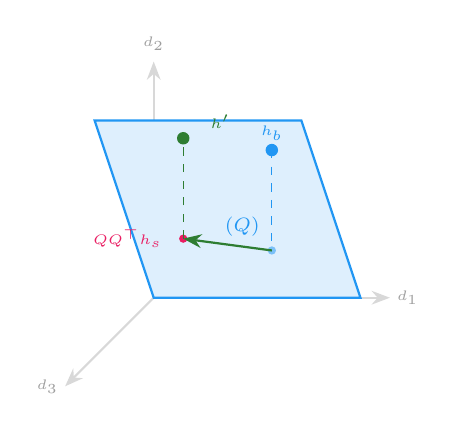
\begin{tikzpicture}[scale=0.75]
  % 3D-ish activation space
  \draw[neutral!40,thick,-{Stealth}] (0,0) -- (4,0);
  \draw[neutral!40,thick,-{Stealth}] (0,0) -- (0,4);
  \draw[neutral!40,thick,-{Stealth}] (0,0) -- (-1.5,-1.5);
  \node[font=\tiny,neutral] at (4.3,0) {$d_1$};
  \node[font=\tiny,neutral] at (0,4.3) {$d_2$};
  \node[font=\tiny,neutral] at (-1.8,-1.5) {$d_3$};

  % The subspace (a plane)
  \fill[das!15] (0,0) -- (3.5,0) -- (2.5,3) -- (-1,3) -- cycle;
  \draw[das,thick] (0,0) -- (3.5,0) -- (2.5,3) -- (-1,3) -- cycle;
  \node[font=\scriptsize,das] at (1.5,1.2) {$\Span(Q)$};

  % Base point
  \fill[das] (2,2.5) circle (3pt);
  \node[font=\tiny,das,above] at (2,2.5) {$h_b$};

  % Projection
  \draw[das,dashed] (2,2.5) -- (2,0.8);
  \fill[das!60] (2,0.8) circle (2pt);

  % Source projection
  \fill[circle] (0.5,1.0) circle (2pt);
  \node[font=\tiny,circle,left] at (0.3,1.0) {$QQ^\top h_s$};

  % Intervened point
  \draw[grass,thick,-{Stealth}] (2,0.8) -- (0.5,1.0);
  \fill[grass] (2,2.5) ++(-1.5,0.2) circle (3pt);
  \node[font=\tiny,grass,above right] at (0.8,2.7) {$h'$};
  \draw[grass,dashed] (0.5,1.0) -- (0.5,2.7);
\end{tikzpicture}

\vspace{0.3em}
\centering
{\scriptsize DAS projects onto a \textbf{flat plane}.\\What if the variable lives on a \textbf{curve}?}
\end{column}
\end{columns}
\end{frame}

%% --- SLIDE: The Grassmannian (original) ---
\begin{frame}{The Grassmannian manifold $\Gr(k,d)$}

\begin{columns}[T]
\begin{column}{0.62\textwidth}
{\small The Grassmannian $\Gr(k,d)$ is the set of all $k$-dimensional linear subspaces of $\R^d$.}

\vspace{0.3em}
{\small Think of it as a ``space of planes.'' Every DAS solution picks one plane from this space. The distance between two planes is measured by their \textbf{principal angles}:}

\vspace{-2pt}
{\small $$d_{\Gr}([Q_1],[Q_2]) = \textstyle\left(\sum_i \theta_i^2\right)^{1/2}$$}

\vspace{-6pt}
{\small When we ask ``does DAS work?'' we are really asking:}

\vspace{0.2em}
\begin{center}
\fcolorbox{grass}{grass!10}{\parbox{0.88\linewidth}{\centering\vspace{0.2em}
  {\small Does the true causal variable live on $\Gr(k,d)$?}
\vspace{0.2em}}}
\end{center}

\vspace{0.2em}
{\small If yes: DAS finds a meaningful point.\\
If no: DAS still returns a point, but it is an \textbf{artifact}.}
\end{column}
\begin{column}{0.36\textwidth}
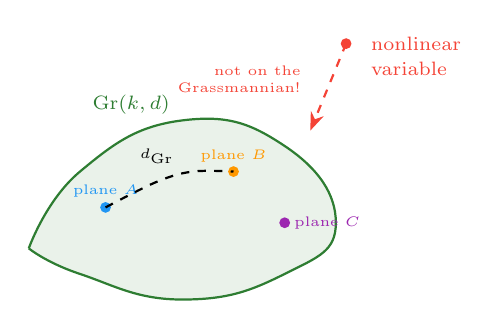
\begin{tikzpicture}[scale=0.65]
  % Grassmannian as a curved surface
  \draw[grass,thick,fill=grass!10]
    plot[smooth,tension=0.8] coordinates {(-2,0) (-1,1.5) (1,2.5) (3,2) (4,0.5) (3,-0.5) (1,-1) (-1,-0.5) (-2,0)};
  \node[font=\scriptsize\bfseries,grass] at (0,2.8) {$\Gr(k,d)$};

  % Points on it = different subspaces
  \fill[das] (-0.5,0.8) circle (3pt);
  \node[font=\tiny,das,above] at (-0.5,0.8) {plane $A$};

  \fill[stoch] (2,1.5) circle (3pt);
  \node[font=\tiny,stoch,above] at (2,1.5) {plane $B$};

  \fill[vae] (3,0.5) circle (3pt);
  \node[font=\tiny,vae,right] at (3,0.5) {plane $C$};

  % Geodesic
  \draw[black,thick,dashed]
    plot[smooth,tension=0.6] coordinates {(-0.5,0.8) (0.5,1.3) (1.2,1.5) (2,1.5)};
  \node[font=\tiny] at (0.5,1.8) {$d_{\Gr}$};

  % Off-manifold point — moved to the right
  \fill[never] (4.2,4.0) circle (3pt);
  \node[font=\scriptsize,never,right] at (4.5,4.0) {nonlinear};
  \node[font=\scriptsize,never,right] at (4.5,3.5) {variable};
  \draw[never,thick,dashed,-{Stealth}] (4.2,4.0) -- (3.5,2.3);
  \node[font=\tiny,never,left,align=right] at (3.5,3.3) {not on the\\Grassmannian!};
\end{tikzpicture}

\vspace{0.3em}
\centering
{\scriptsize A nonlinear causal variable (circle, sphere)\\does not live on $\Gr(k,d)$ at any $k$.}
\end{column}
\end{columns}
\end{frame}

\hypertarget{sec3}{}
\section{3. Why linearity matters}

%% --- SLIDE: Linear vs nonlinear causal variables ---
\begin{frame}{Linear vs.\ nonlinear causal variables}

\begin{columns}[T]
\begin{column}{0.48\textwidth}
\centering
\textbf{\textcolor{das}{Linear causal variable}}

\vspace{0.3em}
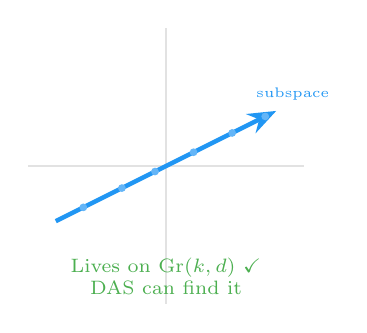
\begin{tikzpicture}[scale=0.7]
  \draw[neutral!30] (-2.5,0) -- (2.5,0);
  \draw[neutral!30] (0,-2.5) -- (0,2.5);

  % Linear subspace
  \draw[das,ultra thick,-{Stealth}] (-2,-1) -- (2,1);
  \node[font=\tiny,das] at (2.3,1.3) {subspace};

  % Points projected onto line
  \foreach \x/\y in {-1.5/-0.75, -0.8/-0.4, -0.2/-0.1, 0.5/0.25, 1.2/0.6, 1.8/0.9} {
    \fill[das!70] (\x,\y) circle (2pt);
  }

  \node[font=\scriptsize,pass,align=center] at (0,-2) {Lives on $\Gr(k,d)$ \checkmark\\DAS can find it};
\end{tikzpicture}

\vspace{0.3em}
{\small Examples: IOI indirect object (partially), multiplication mod $p$ after grokking}
\end{column}
\begin{column}{0.48\textwidth}
\centering
\textbf{\textcolor{circle}{Nonlinear causal variable}}

\vspace{0.3em}
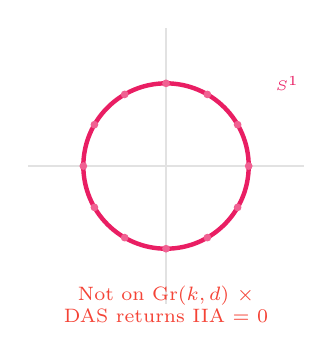
\begin{tikzpicture}[scale=0.7]
  \draw[neutral!30] (-2.5,0) -- (2.5,0);
  \draw[neutral!30] (0,-2.5) -- (0,2.5);

  % Circle
  \draw[circle,ultra thick] (0,0) circle (1.5);

  % Points on circle
  \foreach \a in {0,30,...,330} {
    \fill[circle!70] ({1.5*cos(\a)},{1.5*sin(\a)}) circle (2pt);
  }
  \node[font=\tiny,circle] at (2.2,1.5) {$S^1$};

  \node[font=\scriptsize,fail,align=center] at (0,-2.5) {Not on $\Gr(k,d)$ $\times$\\DAS returns IIA = 0};
\end{tikzpicture}

\vspace{0.3em}
{\small Examples: addition mod $p$ after grokking (Fourier representation encodes numbers on a circle)}
\end{column}
\end{columns}
\end{frame}

%% --- SLIDE: The central question ---
\begin{frame}{The central question}

\begin{center}
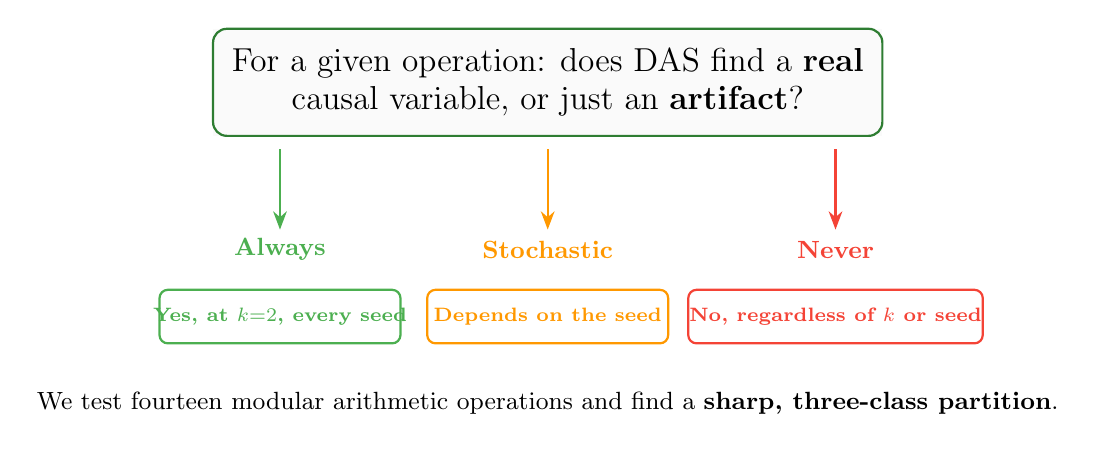
\begin{tikzpicture}[scale=0.85]
  % Question box
  \fill[bg] (-5,-0.8) rectangle (5,0.8);
  \draw[grass,thick,rounded corners=5pt] (-5,-0.8) rectangle (5,0.8);
  \node[font=\large,align=center] at (0,0) {For a given operation: does DAS find a \textbf{real}\\causal variable, or just an \textbf{artifact}?};

  % Three possibilities
  \node[font=\small\bfseries,always] at (-4,-2.5) {Always};
  \draw[always,thick,rounded corners=3pt] (-5.8,-3.1) rectangle (-2.2,-3.9);
  \node[font=\scriptsize,always,align=center] at (-4,-3.5) {\textbf{Yes, at $k{=}2$, every seed}};

  \node[font=\small\bfseries,stoch] at (0,-2.5) {Stochastic};
  \draw[stoch,thick,rounded corners=3pt] (-1.8,-3.1) rectangle (1.8,-3.9);
  \node[font=\scriptsize,stoch,align=center] at (0,-3.5) {\textbf{Depends on the seed}};

  \node[font=\small\bfseries,never] at (4.3,-2.5) {Never};
  \draw[never,thick,rounded corners=3pt] (2.1,-3.1) rectangle (6.5,-3.9);
  \node[font=\scriptsize,never,align=center] at (4.3,-3.5) {\textbf{No, regardless of $k$ or seed}};

  % Arrows
  \draw[always,thick,-{Stealth}] (-4,-1.0) -- (-4,-2.2);
  \draw[stoch,thick,-{Stealth}] (0,-1.0) -- (0,-2.2);
  \draw[never,thick,-{Stealth}] (4.3,-1.0) -- (4.3,-2.2);

  % Bottom line
  \node[font=\small,align=center] at (0,-4.8) {We test fourteen modular arithmetic operations and find a \textbf{sharp, three-class partition}.};
\end{tikzpicture}
\end{center}
\end{frame}

%% --- SLIDE: Why subspaces matter for circuits ---
\begin{frame}{Why subspaces matter for circuits}

\begin{columns}[T]
\begin{column}{0.48\textwidth}
{\small Mechanistic interpretability asks two questions about neural network circuits:}

\vspace{0.5em}
\textbf{\textcolor{das}{Q1: Which components?}}\\[0.2em]
{\small Which attention heads and MLPs matter for a behavior? Which edges carry the signal?}

\vspace{0.3em}
{\footnotesize Methods: activation patching, attribution patching, EAP.}

\vspace{0.5em}
\textbf{\textcolor{vae}{Q2: What do they communicate?}}\\[0.2em]
{\small When two components are connected, \emph{what} flows between them? Which subspaces of the residual stream carry the signal?}

\vspace{0.3em}
{\footnotesize Methods: DAS, probing, SAEs.}
\end{column}
\begin{column}{0.48\textwidth}
\vspace{0.5em}
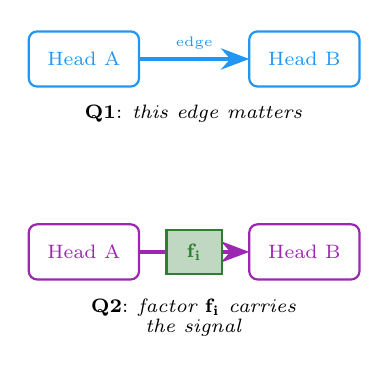
\begin{tikzpicture}[scale=0.7]
  % Edge (Q1)
  \draw[das,thick,rounded corners=3pt] (-1,4.5) rectangle (1,5.5);
  \node[font=\scriptsize,das] at (0,5.0) {Head A};
  \draw[das,thick,rounded corners=3pt] (3,4.5) rectangle (5,5.5);
  \node[font=\scriptsize,das] at (4,5.0) {Head B};
  \draw[das,ultra thick,-{Stealth}] (1,5.0) -- (3,5.0);
  \node[font=\tiny,das,above] at (2,5.0) {edge};
  \node[font=\scriptsize] at (2,4.0) {\textbf{Q1}: \emph{this edge matters}};

  % Subspace (Q2)
  \draw[vae,thick,rounded corners=3pt] (-1,1.0) rectangle (1,2.0);
  \node[font=\scriptsize,vae] at (0,1.5) {Head A};
  \draw[vae,thick,rounded corners=3pt] (3,1.0) rectangle (5,2.0);
  \node[font=\scriptsize,vae] at (4,1.5) {Head B};
  \draw[vae,ultra thick,-{Stealth}] (1,1.5) -- (3,1.5);
  \fill[grass!30] (1.5,1.1) rectangle (2.5,1.9);
  \draw[grass,thick] (1.5,1.1) rectangle (2.5,1.9);
  \node[font=\scriptsize,grass] at (2,1.5) {$\mathbf{f_i}$};
  \node[font=\scriptsize,align=center] at (2,0.3) {\textbf{Q2}: \emph{factor $\mathbf{f_i}$ carries}\\[-0.1em]\emph{the signal}};
\end{tikzpicture}

\vspace{0.3em}
\fcolorbox{grass}{grass!10}{\parbox{0.9\linewidth}{\centering\vspace{0.2em}
  {\small Our work: whether Q2 has a \textbf{linear} answer depends on the operation.}
\vspace{0.2em}}}
\end{column}
\end{columns}

\end{frame}


%% ============================================================
%% PART 2: THE ATLAS
%% ============================================================

\begin{frame}[plain]
\vfill
\begin{center}
  \setlength{\fboxrule}{2.5pt}%
  \fcolorbox{black}{white}{\parbox{0.7\textwidth}{\centering\vspace{0.8em}
    {\Large\bfseries Part 2}\hypertarget{part2}{}\\[0.5em]
    {\large The atlas: fourteen operations, three classes}
  \vspace{0.8em}}}
\end{center}
\vfill
\end{frame}

\begin{frame}{In this section}
\begin{columns}[T]
\begin{column}{0.48\textwidth}
\textbf{\hyperlink{sec4}{4. Fourteen operations, three classes}}\\[0.2em]
{\small We train on 14 modular arithmetic operations and find a sharp partition into three classes based on whether DAS finds a genuine causal variable.}

\vspace{0.6em}
\textbf{\hyperlink{sec5}{5. Linear DAS fails completely}}\\[0.2em]
{\small On grokked addition, DAS returns IIA $= 0$ at every $k$. The Fourier representation lives on $S^1$, not on $\mathrm{Gr}(k,d)$.}
\end{column}
\begin{column}{0.48\textwidth}
\textbf{\hyperlink{sec6}{6. Stochastic grokking}}\\[0.2em]
{\small Power and composite addition grok stochastically: same operation, same hyperparameters, opposite outcomes from different random seeds.}
\end{column}
\end{columns}
\end{frame}

\hypertarget{sec4}{}
\section{4. Fourteen operations, three classes}

%% --- SLIDE: Experimental setup ---
\begin{frame}{Experimental setup}

\begin{columns}[T]
\begin{column}{0.55\textwidth}
{\small We train single-layer transformers on modular arithmetic:}

\vspace{0.2em}
{\small Input: $(a, b, {=})$ \quad Output: $f(a,b) \bmod p$}

\vspace{0.3em}
{\small Model: $d_\text{model} = 128$, 4 heads, standard grokking setup (30\% train, AdamW, weight decay 1.0).}

\vspace{0.3em}
{\small For each trained model, we:}
\begin{enumerate}
  \item {\small Cache residual-stream activations}
  \item {\small Train DAS at $k \in \{2, 4, 6, \ldots, 32\}$}
  \item {\small Measure IIA, equivariance, circle geometry}
  \item {\small Train a structured VAE}
\end{enumerate}

\vspace{0.3em}
{\small 14 operations spanning group actions, polynomials, piecewise, and non-algebraic maps.}
\end{column}
\begin{column}{0.42\textwidth}
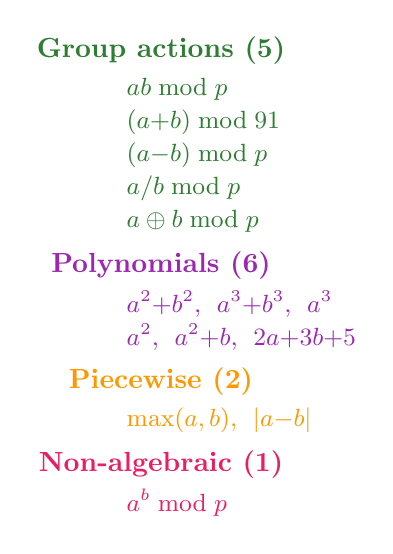
\begin{tikzpicture}[scale=0.7]
  % Operation categories
  \node[font=\normalsize\bfseries,grass] at (0,6.5) {Group actions (\textbf{5})};
  \node[font=\small,grass,anchor=west] at (-0.8,5.8) {$ab \bmod p$};
  \node[font=\small,grass,anchor=west] at (-0.8,5.2) {$(a{+}b) \bmod 91$};
  \node[font=\small,grass,anchor=west] at (-0.8,4.6) {$(a{-}b) \bmod p$};
  \node[font=\small,grass,anchor=west] at (-0.8,4.0) {$a/b \bmod p$};
  \node[font=\small,grass,anchor=west] at (-0.8,3.4) {$a \oplus b \bmod p$};

  \node[font=\normalsize\bfseries,vae] at (0,2.6) {Polynomials (\textbf{6})};
  \node[font=\small,vae,anchor=west] at (-0.8,1.9) {$a^2{+}b^2$,\; $a^3{+}b^3$,\; $a^3$};
  \node[font=\small,vae,anchor=west] at (-0.8,1.3) {$a^2$,\; $a^2{+}b$,\; $2a{+}3b{+}5$};

  \node[font=\normalsize\bfseries,nldas] at (0,0.5) {Piecewise (\textbf{2})};
  \node[font=\small,nldas,anchor=west] at (-0.8,-0.2) {$\max(a,b)$,\; $|a{-}b|$};

  \node[font=\normalsize\bfseries,circle] at (0,-1.0) {Non-algebraic (\textbf{1})};
  \node[font=\small,circle,anchor=west] at (-0.8,-1.7) {$a^b \bmod p$};
\end{tikzpicture}
\end{column}
\end{columns}
\end{frame}

%% --- SLIDE: What is grokking ---
\begin{frame}{What is grokking?}

\begin{columns}[T]
\begin{column}{0.55\textwidth}
{\small \textbf{Grokking} is a training phenomenon where models memorize the training set long before they generalize.}%
\footnote{\tiny Power et al., ``Grokking: Generalization Beyond Overfitting on Small Algorithmic Datasets,'' 2022.}

\vspace{0.3em}
{\small For modular arithmetic with weight decay:}
\begin{itemize}
  \item {\small Train loss drops to zero quickly (memorization)}
  \item {\small Test loss stays high for thousands of epochs}
  \item {\small Then suddenly drops (generalization)}
\end{itemize}

\vspace{0.3em}
{\small The internal representation changes during grokking: from a lookup table (memorization) to a structured algorithm (Fourier representation).}

\vspace{0.3em}
{\small Prior work showed grokked models use Fourier features\footnote{\tiny Nanda et al., ``Progress Measures for Grokking via Mechanistic Interpretability,'' ICLR 2023.}:\\$a \mapsto (\cos 2\pi f a / p, \sin 2\pi f a / p)$}

\vspace{0.3em}
{\small Our contribution: \textbf{grokking determines whether the causal variable is Grassmannian.}}
\end{column}
\begin{column}{0.42\textwidth}
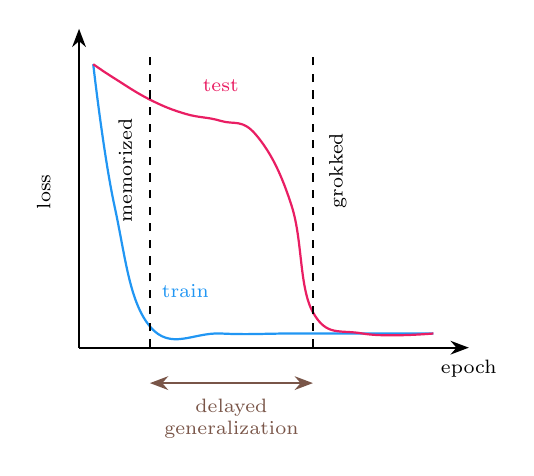
\begin{tikzpicture}[scale=0.9]
  % Training curve
  \draw[black,thick,-{Stealth}] (0,0) -- (5.5,0);
  \draw[black,thick,-{Stealth}] (0,0) -- (0,4.5);
  \node[font=\scriptsize] at (5.5,-0.3) {epoch};
  \node[font=\scriptsize,rotate=90] at (-0.5,2.2) {loss};

  % Train loss
  \draw[das,thick] plot[smooth,tension=0.7] coordinates {(0.2,4) (0.5,2) (1,0.3) (2,0.2) (3,0.2) (4,0.2) (5,0.2)};
  \node[font=\scriptsize,das] at (1.5,0.8) {train};

  % Test loss (grokking)
  \draw[circle,thick] plot[smooth,tension=0.7] coordinates {(0.2,4) (0.5,3.8) (1,3.5) (1.5,3.3) (2,3.2) (2.5,3.0) (3,2) (3.3,0.5) (4,0.2) (5,0.2)};
  \node[font=\scriptsize,circle] at (2,3.7) {test};

  % Annotations
  \draw[black,thick,dashed] (1,0) -- (1,4.2);
  \node[font=\scriptsize,align=center,rotate=90] at (0.65,2.5) {memorized};

  \draw[black,thick,dashed] (3.3,0) -- (3.3,4.2);
  \node[font=\scriptsize,align=center,rotate=90] at (3.65,2.5) {grokked};

  % Phase labels
  \draw[{Stealth}-{Stealth},memo,thick] (1,-0.5) -- (3.3,-0.5);
  \node[font=\scriptsize,memo,align=center] at (2.15,-1.0) {delayed\\generalization};
\end{tikzpicture}
\end{column}
\end{columns}
\end{frame}

%% --- SLIDE: The atlas results ---
\begin{frame}{The atlas: three sharp classes}
\centering
\vspace{-0.5em}
{\footnotesize\setlength{\tabcolsep}{2.5pt}\renewcommand{\arraystretch}{0.92}
\begin{tabular}{lcccccl}
\toprule
\textbf{Operation} & \textbf{Grok} & \textbf{Loss} & \textbf{IIA}($k{=}2$) & $\boldsymbol{k^*}$ & \textbf{Equiv.} & \textbf{Class} \\
\midrule
Multiplication & \checkmark & 0.000 & 1.000 & 2 & 0.995 & \textcolor{always}{Always} \\
Subtraction & \checkmark & 0.000 & 1.000 & 2 & 1.000 & \textcolor{always}{Always} \\
Division & \checkmark & 0.000 & 1.000 & 2 & 1.000 & \textcolor{always}{Always} \\
Bitwise XOR & \checkmark & 0.003 & 1.000 & 2 & 1.000 & \textcolor{always}{Always} \\
Cubic sum & \checkmark & 0.000 & 1.000 & 2 & 1.000 & \textcolor{always}{Always} \\
Sum of squares & \checkmark & 0.005 & 1.000 & 2 & 0.987 & \textcolor{always}{Always} \\
Max & \checkmark & 0.074 & 0.960 & 2 & 0.957 & \textcolor{always}{Always} \\
\midrule
Power (s137) & \checkmark & 0.088 & 0.940 & 4 & 0.965 & \textcolor{stoch}{Stochastic} \\
Power (s42) & $\times$ & 1.143 & 0.980 & 2 & 0.665 & \textcolor{stoch}{Stochastic} \\
Comp.\ add.\ (orig) & \checkmark & 0.002 & 1.000 & 2 & 0.998 & \textcolor{stoch}{Stochastic} \\
Comp.\ add.\ (s42) & $\times$ & 10.21 & 0.800 & ${>}32$ & 0.110 & \textcolor{stoch}{Stochastic} \\
\midrule
Cubing & $\times$ & 9.765 & 0.857 & 4 & 0.509 & \textcolor{never}{Never} \\
Squaring & $\times$ & 7.808 & 0.857 & 4 & 0.314 & \textcolor{never}{Never} \\
Abs.\ difference & $\times$ & 1.835 & 0.800 & ${>}32$ & 0.189 & \textcolor{never}{Never} \\
Polynomial & $\times$ & 21.55 & 0.720 & ${>}32$ & 0.015 & \textcolor{never}{Never} \\
Affine & $\times$ & 26.21 & 0.780 & ${>}32$ & 0.026 & \textcolor{never}{Never} \\
\bottomrule
\end{tabular}}

\vspace{0.2em}
{\small $k^*$ = smallest $k$ where IIA $\geq 0.95$. Equiv.\ = equivariance under additive shift.}
\end{frame}

%% --- SLIDE: Loss vs equivariance (real data) ---
\begin{frame}{Loss vs.\ equivariance: grokking is the boundary}
\begin{columns}[T]
\begin{column}{0.55\textwidth}
\vspace{-0.3em}
\includegraphics[width=\linewidth]{fig12_loss_vs_equiv_paper.pdf}
\end{column}
\begin{column}{0.42\textwidth}
\vspace{1em}
{\small Each point is one (operation, seed) pair.}

\vspace{0.3em}
{\small \textbf{\textcolor{always}{Blue}}: grokked models (test loss $< 0.1$).\\
\textbf{\textcolor{never}{Pink}}: non-grokked models.}

\vspace{0.3em}
{\small The boundary is sharp: grokking $\Leftrightarrow$ high equivariance $\Leftrightarrow$ Grassmannian causal variable.}

\vspace{0.3em}
{\small No operation sits in the middle. The three-class partition is not a continuum.}
\end{column}
\end{columns}
\end{frame}

%% --- SLIDE: Sorted equivariance dot plot ---
\begin{frame}{Equivariance across all operations and seeds}
\centering
\vspace{-0.5em}
\includegraphics[width=0.85\linewidth]{fig15d_sorted_dot.pdf}

\vspace{0.3em}
{\small Each dot is one (operation, seed) pair, sorted by equivariance.
The gap between $\sim$52\% and $\sim$95\% is empty --- the partition is \textbf{discrete}, not continuous.}
\end{frame}

%% --- SLIDE: Bridge — grokking predicts geometry ---
\begin{frame}{The finding: grokking predicts geometry}

\begin{center}
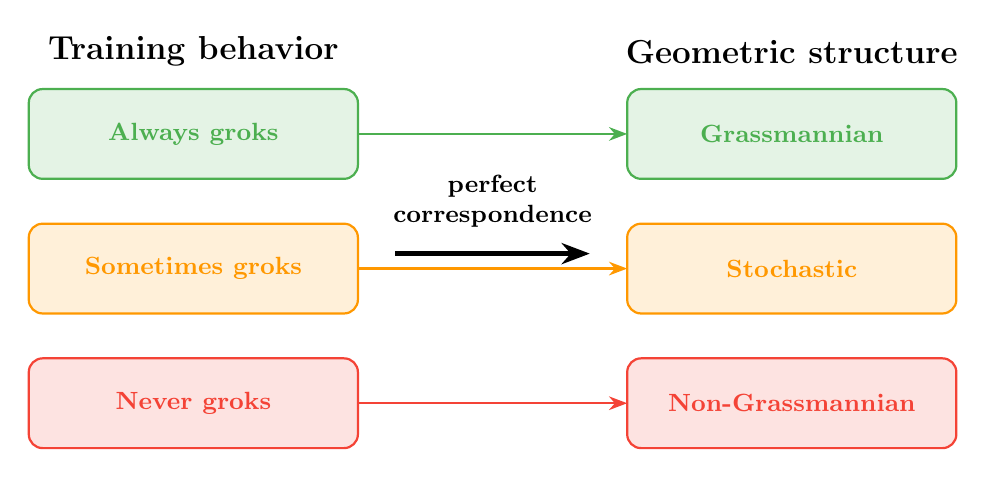
\begin{tikzpicture}[scale=0.95]
  % Left column: training phenomenon
  \node[font=\large\bfseries] at (-4,5.5) {Training behavior};

  \fill[always!15,rounded corners=5pt] (-6.2,3.8) rectangle (-1.8,5.0);
  \draw[always,thick,rounded corners=5pt] (-6.2,3.8) rectangle (-1.8,5.0);
  \node[font=\small\bfseries,always] at (-4,4.4) {Always groks};

  \fill[stoch!15,rounded corners=5pt] (-6.2,2.0) rectangle (-1.8,3.2);
  \draw[stoch,thick,rounded corners=5pt] (-6.2,2.0) rectangle (-1.8,3.2);
  \node[font=\small\bfseries,stoch] at (-4,2.6) {Sometimes groks};

  \fill[never!15,rounded corners=5pt] (-6.2,0.2) rectangle (-1.8,1.4);
  \draw[never,thick,rounded corners=5pt] (-6.2,0.2) rectangle (-1.8,1.4);
  \node[font=\small\bfseries,never] at (-4,0.8) {Never groks};

  % Arrow
  \draw[black,ultra thick,-{Stealth}] (-1.3,2.8) -- (1.3,2.8);
  \node[font=\small\bfseries,align=center] at (0,3.5) {perfect\\correspondence};

  % Right column: geometric structure
  \node[font=\large\bfseries] at (4,5.5) {Geometric structure};

  \fill[always!15,rounded corners=5pt] (1.8,3.8) rectangle (6.2,5.0);
  \draw[always,thick,rounded corners=5pt] (1.8,3.8) rectangle (6.2,5.0);
  \node[font=\small\bfseries,always] at (4,4.4) {Grassmannian};

  \fill[stoch!15,rounded corners=5pt] (1.8,2.0) rectangle (6.2,3.2);
  \draw[stoch,thick,rounded corners=5pt] (1.8,2.0) rectangle (6.2,3.2);
  \node[font=\small\bfseries,stoch] at (4,2.6) {Stochastic};

  \fill[never!15,rounded corners=5pt] (1.8,0.2) rectangle (6.2,1.4);
  \draw[never,thick,rounded corners=5pt] (1.8,0.2) rectangle (6.2,1.4);
  \node[font=\small\bfseries,never] at (4,0.8) {Non-Grassmannian};

  % Connecting arrows
  \draw[always,thick,-{Stealth}] (-1.8,4.4) -- (1.8,4.4);
  \draw[stoch,thick,-{Stealth}] (-1.8,2.6) -- (1.8,2.6);
  \draw[never,thick,-{Stealth}] (-1.8,0.8) -- (1.8,0.8);
\end{tikzpicture}
\end{center}

\vspace{0.3em}
{\small Grokking is the mechanism: when generalization happens, the representation becomes a linear subspace on $\Gr(k,d)$. When it doesn't, the variable stays nonlinear.}
\end{frame}

%% --- SLIDE: Visual summary of classes ---
\begin{frame}{Three classes, one mechanism}

\vspace{-0.5em}
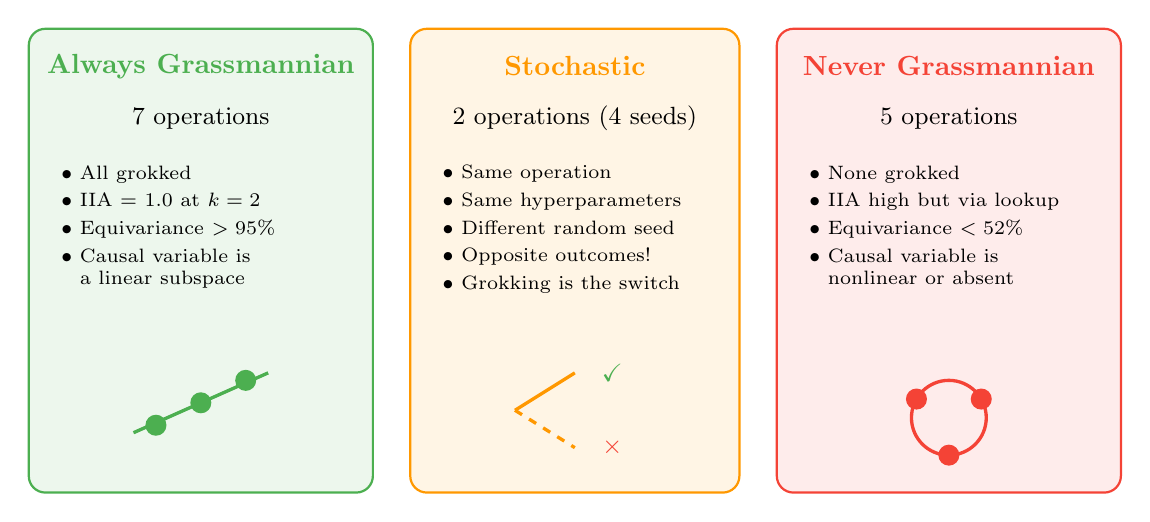
\begin{tikzpicture}[scale=0.95]
  % Always
  \fill[always!10,rounded corners=6pt] (-5.8,-1.0) rectangle (-1.2,5.2);
  \draw[always,thick,rounded corners=6pt] (-5.8,-1.0) rectangle (-1.2,5.2);
  \node[font=\normalsize\bfseries,always] at (-3.5,4.7) {Always Grassmannian};
  \node[font=\small,align=center] at (-3.5,4.0) {7 operations};
  \node[font=\scriptsize,align=left,anchor=north west] at (-5.5,3.5) {%
    $\bullet$ All grokked\\[2pt]
    $\bullet$ IIA = 1.0 at $k = 2$\\[2pt]
    $\bullet$ Equivariance $> 95\%$\\[2pt]
    $\bullet$ Causal variable is\\
    \phantom{$\bullet$} a linear subspace};
  % Mini diagram — lower
  \draw[always,very thick] (-4.4,-0.2) -- (-2.6,0.6);
  \fill[always] (-4.1,-0.1) circle (4pt);
  \fill[always] (-3.5,0.2) circle (4pt);
  \fill[always] (-2.9,0.5) circle (4pt);

  % Stochastic
  \fill[stoch!10,rounded corners=6pt] (-0.7,-1.0) rectangle (3.7,5.2);
  \draw[stoch,thick,rounded corners=6pt] (-0.7,-1.0) rectangle (3.7,5.2);
  \node[font=\normalsize\bfseries,stoch] at (1.5,4.7) {Stochastic};
  \node[font=\small,align=center] at (1.5,4.0) {2 operations (4 seeds)};
  \node[font=\scriptsize,align=left,anchor=north west] at (-0.4,3.5) {%
    $\bullet$ Same operation\\[2pt]
    $\bullet$ Same hyperparameters\\[2pt]
    $\bullet$ Different random seed\\[2pt]
    $\bullet$ Opposite outcomes!\\[2pt]
    $\bullet$ Grokking is the switch};
  % Mini diagram: coin flip — lower
  \draw[stoch,very thick] (0.7,0.1) -- (1.5,0.6);
  \draw[stoch,very thick,dashed] (0.7,0.1) -- (1.5,-0.4);
  \node[font=\small,always] at (2.0,0.6) {\checkmark};
  \node[font=\small,never] at (2.0,-0.4) {$\times$};

  % Never
  \fill[never!10,rounded corners=6pt] (4.2,-1.0) rectangle (8.8,5.2);
  \draw[never,thick,rounded corners=6pt] (4.2,-1.0) rectangle (8.8,5.2);
  \node[font=\normalsize\bfseries,never] at (6.5,4.7) {Never Grassmannian};
  \node[font=\small,align=center] at (6.5,4.0) {5 operations};
  \node[font=\scriptsize,align=left,anchor=north west] at (4.5,3.5) {%
    $\bullet$ None grokked\\[2pt]
    $\bullet$ IIA high but via lookup\\[2pt]
    $\bullet$ Equivariance $< 52\%$\\[2pt]
    $\bullet$ Causal variable is\\
    \phantom{$\bullet$} nonlinear or absent};
  % Mini diagram: circle — lower
  \draw[never,very thick] (6.5,0.0) circle (0.5);
  \fill[never] ({6.5+0.5*cos(30)},{0.0+0.5*sin(30)}) circle (4pt);
  \fill[never] ({6.5+0.5*cos(150)},{0.0+0.5*sin(150)}) circle (4pt);
  \fill[never] ({6.5+0.5*cos(270)},{0.0+0.5*sin(270)}) circle (4pt);
\end{tikzpicture}
\end{frame}

\hypertarget{sec5}{}
\section{5. Linear DAS fails completely}

%% --- SLIDE: DAS = 0 on addition ---
\begin{frame}{Linear DAS returns zero IIA on grokked modular addition}

\begin{columns}[T]
\begin{column}{0.58\textwidth}
{\small Standard addition mod 113 (prime) groks perfectly (test loss $< 10^{-7}$). The model has learned the correct algorithm.}

\vspace{0.3em}
{\small But DAS returns $\IIA = 0.0$ at \textbf{every} subspace dimension $k \in \{2, 4, 8, 16\}$.}

\vspace{0.3em}
{\small This is not an optimization failure. The model encodes numbers using Fourier features:}

\vspace{-4pt}
{\small $$a \mapsto (\cos \tfrac{2\pi f a}{p},\; \sin \tfrac{2\pi f a}{p})$$}

\vspace{-6pt}
{\small This representation lives on a \textbf{circle} $S^1$ in $\R^d$, not a linear subspace.}

\vspace{0.2em}
{\small DAS searches $\Gr(k,d)$ for a flat plane that captures a curved manifold --- a \textbf{category error}, not an optimization failure.}
\end{column}
\begin{column}{0.39\textwidth}
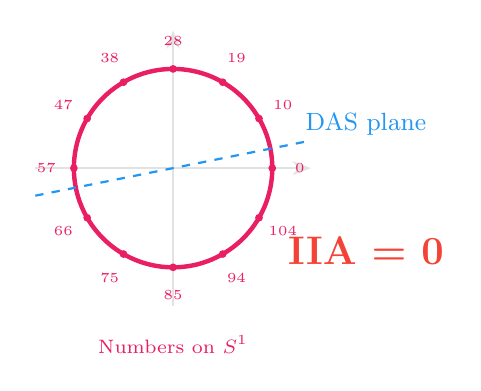
\begin{tikzpicture}[scale=0.7]
  % Circle in activation space
  \draw[neutral!30,thick,-{Stealth}] (-2.5,0) -- (2.5,0);
  \draw[neutral!30,thick,-{Stealth}] (0,-2.5) -- (0,2.5);

  % The circle
  \draw[circle,ultra thick] (0,0) circle (1.8);

  % Points labeled with numbers
  \foreach \a/\lab in {0/0, 30/10, 60/19, 90/28, 120/38, 150/47, 180/57, 210/66, 240/75, 270/85, 300/94, 330/104} {
    \fill[circle] ({1.8*cos(\a)},{1.8*sin(\a)}) circle (2pt);
    \node[font=\tiny,circle] at ({2.3*cos(\a)},{2.3*sin(\a)}) {\lab};
  }

  \node[font=\scriptsize,circle] at (0,-3.2) {Numbers on $S^1$};

  % A linear subspace cutting through
  \draw[das,thick,dashed] (-2.5,-0.5) -- (2.5,0.5);
  \node[font=\small,das] at (3.5,0.8) {DAS plane};

  % IIA = 0 — moved right
  \node[font=\Large,fail] at (3.5,-1.5) {\textbf{IIA = 0}};
\end{tikzpicture}
\end{column}
\end{columns}
\end{frame}

%% --- SLIDE: k-sweep profiles ---
\begin{frame}{$k$-sweep profiles distinguish the three classes}

\begin{columns}[T]
\begin{column}{0.50\textwidth}
\vspace{-0.5em}
\includegraphics[width=\linewidth]{fig14_k_sweep.pdf}
\end{column}
\begin{column}{0.46\textwidth}
\vspace{1em}
{\small \textbf{Always Grassmannian}: IIA saturates at 1.0 by $k = 2$. The causal variable is intrinsically 2-dimensional.}

\vspace{0.5em}
{\small \textbf{Stochastic}: power jumps to 1.0 at $k = 4$, depending on seed.}

\vspace{0.5em}
{\small \textbf{Never Grassmannian}: IIA rises gradually and may not reach 1.0 even at $k = 32$. More dimensions help, but the fit is never clean.}

\vspace{0.5em}
{\small The $k$-sweep profile is a \textbf{diagnostic}: if IIA keeps rising past $k = 4$, the causal variable is probably not Grassmannian.}
\end{column}
\end{columns}
\end{frame}

\hypertarget{sec6}{}
\section{6. Stochastic grokking}

%% --- SLIDE: Stochastic grokking ---
\begin{frame}{Stochastic grokking: same operation, opposite outcomes}

\begin{columns}[T]
\begin{column}{0.55\textwidth}
{\small The stochastic class is the \textbf{strongest evidence}:}

\vspace{0.3em}
{\small \textbf{Power} ($a^b \bmod 113$):}
\begin{itemize}
  \item {\small Seed 137: grokked. Equiv = 96.5\%}
  \item {\small Seed 42: not grokked. Equiv = 66.5\%}
\end{itemize}

\vspace{0.3em}
{\small \textbf{Composite addition} ($(a+b) \bmod 91$):}
\begin{itemize}
  \item {\small Original seed: grokked. Equiv = 99.8\%}
  \item {\small Seed 42: not grokked. Equiv = 11.0\%}
\end{itemize}

\vspace{0.3em}
{\small Same operation. Same architecture. Same hyperparameters. \textbf{Opposite outcomes from random initialization alone.}}

\vspace{0.3em}
\fcolorbox{grass}{grass!10}{\parbox{0.9\linewidth}{\centering\vspace{0.2em}
  {\small Grassmannian variables appear if and only if the model generalizes.}
\vspace{0.2em}}}
\end{column}
\begin{column}{0.42\textwidth}
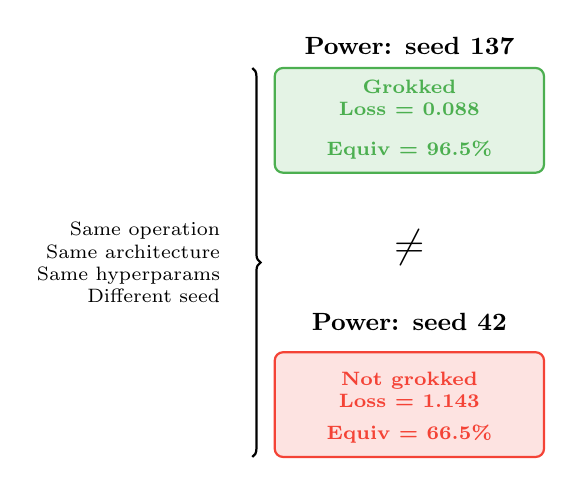
\begin{tikzpicture}[scale=0.95,xshift=-0.6cm]
  % Seed 137
  \node[font=\small\bfseries] at (0,5.5) {Power: seed 137};
  \draw[always,thick,fill=always!15,rounded corners=3pt] (-1.8,3.8) rectangle (1.8,5.2);
  \node[font=\scriptsize\bfseries,always,align=center] at (0,4.8) {Grokked\\Loss = 0.088};
  \node[font=\scriptsize\bfseries,always] at (0,4.1) {Equiv = 96.5\%};

  % Seed 42
  \node[font=\small\bfseries] at (0,1.8) {Power: seed 42};
  \draw[never,thick,fill=never!15,rounded corners=3pt] (-1.8,0.0) rectangle (1.8,1.4);
  \node[font=\scriptsize\bfseries,never,align=center] at (0,0.9) {Not grokked\\Loss = 1.143};
  \node[font=\scriptsize\bfseries,never] at (0,0.3) {Equiv = 66.5\%};

  % Equals sign between
  \node[font=\Large\bfseries] at (0,2.8) {$\neq$};

  % Same everything
  \draw[black,thick,decorate,decoration={brace,mirror,amplitude=3pt}] (-2.1,0.0) -- (-2.1,5.2);
  \node[font=\scriptsize,black,align=right,anchor=east] at (-2.4,2.6) {Same operation\\Same architecture\\Same hyperparams\\Different seed};
\end{tikzpicture}
\end{column}
\end{columns}
\end{frame}

%% --- SLIDE: Equivariance testing ---
\begin{frame}{Equivariance: the geometric diagnostic}

\begin{columns}[T]
\begin{column}{0.48\textwidth}
{\small \textbf{For operations with a group action, the DAS subspace should respect the algebraic symmetry.}}

\vspace{0.3em}
{\small \textbf{Test}: shift input $a \to a + 1 \bmod p$. Does the DAS projection rotate by $\mathbf{2\pi / p}$?}

\vspace{0.3em}
{\small \textbf{Random subspaces}: equivariance $< 1\%$.\\
\textbf{Always Grassmannian}: equivariance $> 95\%$.\\
\textbf{Never Grassmannian}: equivariance $< 52\%$.}

\vspace{0.5em}
{\small \textbf{Equivariance distinguishes:}}
\begin{itemize}
  \item {\small Genuine structure from memorization}
  \item {\small Causal variables from artifacts}
  \item {\small What IIA alone cannot tell apart}
\end{itemize}
\end{column}
\begin{column}{0.50\textwidth}
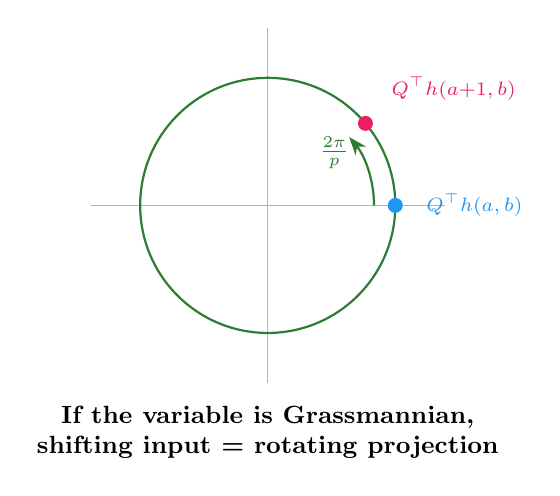
\begin{tikzpicture}[scale=0.9,xshift=-0.5cm]
  \draw[black!30] (-2.5,0) -- (2.5,0);
  \draw[black!30] (0,-2.5) -- (0,2.5);

  % Circle
  \draw[grass,thick] (0,0) circle (1.8);

  % Point at angle 0
  \fill[das] ({1.8*cos(0)},{1.8*sin(0)}) circle (3pt);
  \node[font=\scriptsize\bfseries,das,right] at ({2.1*cos(0)},{2.1*sin(0)}) {$Q^\top h(a,b)$};

  % Point at shifted angle
  \fill[circle] ({1.8*cos(40)},{1.8*sin(40)}) circle (3pt);
  \node[font=\scriptsize\bfseries,circle,above right] at ({2.1*cos(40)},{2.1*sin(40)}) {$Q^\top h(a{+}1,b)$};

  % Rotation arrow
  \draw[grass,thick,-{Stealth}] ({1.5*cos(0)},{1.5*sin(0)})
    arc[start angle=0, end angle=40, radius=1.5];
  \node[font=\small\bfseries,grass] at ({1.0*cos(20)},{1.0*sin(20)+0.4}) {$\frac{2\pi}{p}$};

  % Label
  \node[font=\small\bfseries,align=center] at (0,-3.2) {If the variable is Grassmannian,\\shifting input = rotating projection};
\end{tikzpicture}
\end{column}
\end{columns}
\end{frame}

%% --- SLIDE: Circle geometry (real data) ---
\begin{frame}{Circle geometry: DAS projections reveal structure}
\centering
\vspace{-0.5em}
\includegraphics[width=0.95\linewidth]{fig20_real_circles.pdf}

\vspace{0.2em}
{\small \textbf{\textcolor{always}{Blue}}: grokked operations form clean circles (label centroids on $S^1$).
\textbf{\textcolor{never}{Pink}}: non-grokked operations show random scatter.
Each panel shows the $k{=}2$ DAS projection with per-label centroids overlaid.}
\end{frame}

%% --- SLIDE: Training trajectories (real data) ---
\begin{frame}{Training trajectories: the three classes in action}
\centering
\vspace{-0.5em}
\includegraphics[width=\linewidth]{fig24_three_class_trajectories.pdf}

\vspace{0.3em}
{\small \textbf{A}: Multiplication always groks (all seeds, loss $\to 0$).
\textbf{B}: Power is stochastic (some seeds grok, others plateau).
\textbf{C}: Polynomial never groks (loss stays high across all seeds).
Equivariance values in parentheses track grokking perfectly.}
\end{frame}

%% --- SLIDE: Stochastic trajectories (real data) ---
\begin{frame}{Stochastic grokking: power and composite addition}
\centering
\vspace{-0.5em}
\includegraphics[width=0.85\linewidth]{fig22_stochastic_trajectories.pdf}

\vspace{0.3em}
{\small Multi-seed training for the two stochastic operations. Solid lines with circles = grokked (high equivariance). Dashed lines with diamonds = not grokked (low equivariance). Same operation, same hyperparameters, opposite outcomes from random initialization.}
\end{frame}

%% --- SLIDE: Full k-sweep colored by equivariance ---
\begin{frame}{Full $k$-sweep across all operations}
\centering
\vspace{-0.5em}

\includegraphics[width=0.85\linewidth]{fig23b_k_sweep_equiv_colored.pdf}

\vspace{0.2em}
{\small Each line is one (operation, seed). Color = equivariance (blue = high, red = low).
High-equivariance operations saturate at $k{=}2$; low-equivariance operations rise slowly.
The $k$-sweep is a geometric fingerprint of the causal variable.}
\end{frame}


%% ============================================================
%% PART 3: THE VACUITY PROBLEM
%% ============================================================

\begin{frame}[plain]
\vfill
\begin{center}
  \setlength{\fboxrule}{2.5pt}%
  \fcolorbox{black}{white}{\parbox{0.7\textwidth}{\centering\vspace{0.8em}
    {\Large\bfseries Part 3}\hypertarget{part3}{}\\[0.5em]
    {\large The vacuity problem: when high IIA means nothing}
  \vspace{0.8em}}}
\end{center}
\vfill
\end{frame}

\begin{frame}{In this section}
\begin{columns}[T]
\begin{column}{0.48\textwidth}
\textbf{\hyperlink{sec7}{7. Memorization artifacts}}\\[0.2em]
{\small High IIA does not imply genuine structure. Squaring achieves IIA $= 1.0$ via memorization, exposed by low equivariance.}

\vspace{0.6em}
\textbf{\hyperlink{sec8}{8. Nonlinear DAS is vacuous}}\\[0.2em]
{\small NL-DAS achieves IIA $= 1.0$ on IOI at $k{=}1$ by learning a lookup table. The diversity ratio $\rho \approx 0$ reveals the failure.}
\end{column}
\begin{column}{0.48\textwidth}
\textbf{\hyperlink{sec9}{9. Intervention faithfulness}}\\[0.2em]
{\small We introduce four complementary metrics --- diversity ratio, reconstruction MSE, KL divergence, normalized logit diff --- that distinguish genuine interventions from artifacts.}
\end{column}
\end{columns}
\end{frame}

\hypertarget{sec7}{}
\section{7. Memorization artifacts}

%% --- SLIDE: Memorization produces high IIA ---
\begin{frame}{Memorization produces high IIA}

\begin{columns}[T]
\begin{column}{0.55\textwidth}
{\small Squaring ($a^2 \bmod 113$) achieves $\IIA = 0.86$ at $k = 2$ and $\IIA = 1.0$ by $k = 4$.}

\vspace{0.3em}
{\small But the model \textbf{never grokked} (test loss = 7.8). It memorized the training set.}

\vspace{0.3em}
{\small Equivariance exposes the artifact:}
\begin{itemize}
  \item {\small Squaring: 31.4\% (vs.\ $>95\%$ for genuine)}
  \item {\small Cubing: 50.9\%}
  \item {\small Random subspace: $<1\%$}
\end{itemize}

\vspace{0.5em}
\fcolorbox{fail}{fail!10}{\parbox{0.9\linewidth}{\centering\vspace{0.2em}
  {\small High IIA with low-$k$ saturation is compatible with a \textbf{lookup table}. IIA alone cannot tell the difference.}
\vspace{0.2em}}}
\end{column}
\begin{column}{0.42\textwidth}
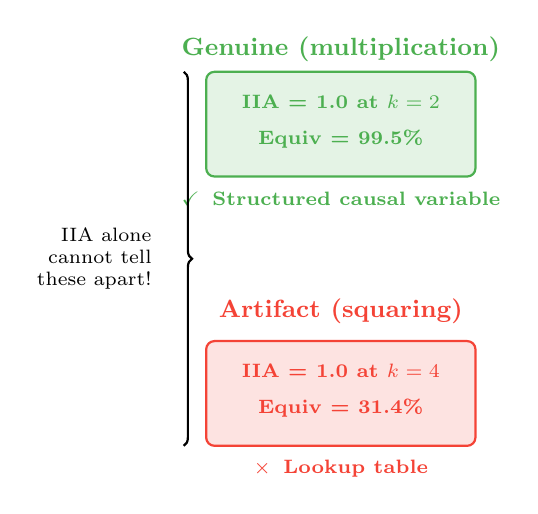
\begin{tikzpicture}[scale=0.95,xshift=-0.6cm]
  % Genuine causal variable
  \node[font=\small\bfseries,always] at (0,5.5) {Genuine (multiplication)};
  \draw[always,thick,fill=always!15,rounded corners=3pt] (-1.8,3.8) rectangle (1.8,5.2);
  \node[font=\scriptsize\bfseries,always,align=center] at (0,4.8) {IIA = 1.0 at $k=2$};
  \node[font=\scriptsize\bfseries,always,align=center] at (0,4.3) {Equiv = 99.5\%};
  \node[font=\scriptsize\bfseries,always] at (0,3.5) {\checkmark\, Structured causal variable};

  % Memorized artifact
  \node[font=\small\bfseries,never] at (0,2.0) {Artifact (squaring)};
  \draw[never,thick,fill=never!15,rounded corners=3pt] (-1.8,0.2) rectangle (1.8,1.6);
  \node[font=\scriptsize\bfseries,never,align=center] at (0,1.2) {IIA = 1.0 at $k=4$};
  \node[font=\scriptsize\bfseries,never,align=center] at (0,0.7) {Equiv = 31.4\%};
  \node[font=\scriptsize\bfseries,never] at (0,-0.1) {$\times$\, Lookup table};

  % The problem
  \draw[black,thick,decorate,decoration={brace,mirror,amplitude=3pt}] (-2.1,0.2) -- (-2.1,5.2);
  \node[font=\scriptsize,black,align=right,anchor=east] at (-2.4,2.7) {IIA alone\\cannot tell\\these apart!};
\end{tikzpicture}
\end{column}
\end{columns}
\end{frame}

\hypertarget{sec8}{}
\section{8. Nonlinear DAS is vacuous}

%% --- SLIDE: The NL-DAS idea ---
\begin{frame}{The natural response: add nonlinearity}

\begin{columns}[T]
\begin{column}{0.55\textwidth}
{\small DAS assumes linearity and fails on nonlinear variables. Natural fix: prepend an MLP featurizer.}

\vspace{0.3em}
{\small \textbf{NL-DAS}: learn encoder $f$ and decoder $g$, then apply linear DAS in the transformed space:}

$$h' = g\bigl(f(h_b) - QQ^\top f(h_b) + QQ^\top f(h_s)\bigr)$$

\vspace{0.3em}
{\small Result on IOI\footnote{\tiny Wang et al., ``Interpretability in the Wild,'' ICLR 2023.} (GPT-2):}
\begin{itemize}
  \item {\small DAS at $k=1$: IIA = 0.193}
  \item {\small NL-DAS at $k=1$: IIA = \textbf{1.000}}
\end{itemize}

\vspace{0.3em}
{\small This looks like a dramatic improvement.}

\vspace{0.3em}
{\normalsize \textbf{It is not.}}
\end{column}
\begin{column}{0.42\textwidth}
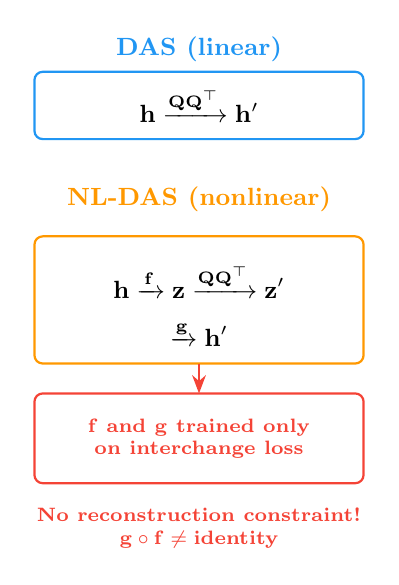
\begin{tikzpicture}[scale=0.95,xshift=-0.3cm]
  % DAS path
  \node[font=\small\bfseries,das] at (0,6.0) {DAS (linear)};
  \draw[das,thick,rounded corners=3pt] (-2.2,4.8) rectangle (2.2,5.7);
  \node[font=\small\bfseries] at (0,5.25) {$\mathbf{h \xrightarrow{QQ^\top} h'}$};

  % NL-DAS path
  \node[font=\small\bfseries,nldas] at (0,4.0) {NL-DAS (nonlinear)};
  \draw[nldas,thick,rounded corners=3pt] (-2.2,1.8) rectangle (2.2,3.5);
  \node[font=\small\bfseries,align=center] at (0,2.9) {$\mathbf{h \xrightarrow{f} z \xrightarrow{QQ^\top} z'}$};
  \node[font=\small\bfseries,align=center] at (0,2.2) {$\mathbf{\xrightarrow{g} h'}$};

  % The problem
  \draw[fail,thick,rounded corners=3pt] (-2.2,0.2) rectangle (2.2,1.4);
  \node[font=\scriptsize\bfseries,fail,align=center] at (0,0.8) {$\mathbf{f}$ and $\mathbf{g}$ trained \textbf{only}\\on interchange loss};

  % Arrow
  \draw[fail,thick,-{Stealth}] (0,1.8) -- (0,1.4);

  \node[font=\scriptsize\bfseries,fail,align=center] at (0,-0.4) {No reconstruction constraint!\\$\mathbf{g \circ f \neq \text{identity}}$};
\end{tikzpicture}
\end{column}
\end{columns}
\end{frame}

%% --- SLIDE: The lookup table failure ---
\begin{frame}{The lookup-table failure mode}

\vspace{-0.3em}
\begin{center}
{\small\bfseries\color{nldas} What NL-DAS actually learns}
\end{center}
\vspace{-0.2em}

\begin{center}
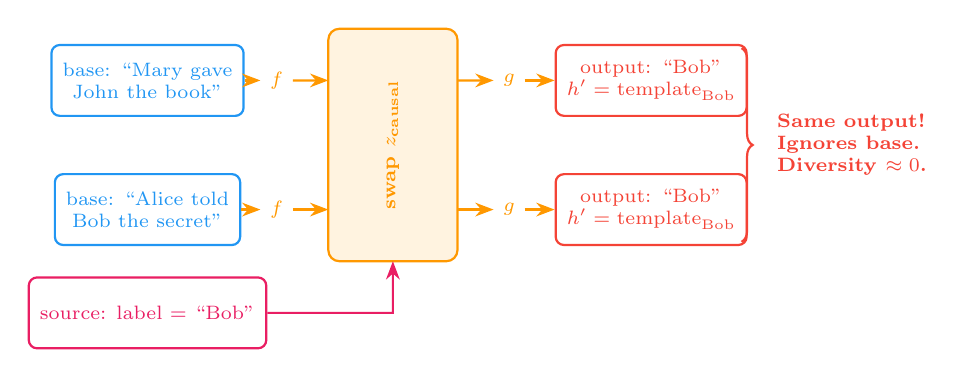
\begin{tikzpicture}[
  scale=0.82,
  box/.style={thick,rounded corners=3pt,minimum height=0.9cm,align=center,font=\scriptsize,inner sep=4pt},
]
  % Row 1: base Mary
  \node[box,draw=das,text=das] (b1) at (-4.2,2.0) {base: ``Mary gave\\John the book''};
  \node[font=\scriptsize\bfseries,nldas] (f1) at (-2.2,2.0) {$f$};
  \draw[nldas,thick,-{Stealth}] (b1.east) -- (f1.west);

  % Row 2: base Alice
  \node[box,draw=das,text=das] (b2) at (-4.2,0.0) {base: ``Alice told\\Bob the secret''};
  \node[font=\scriptsize\bfseries,nldas] (f2) at (-2.2,0.0) {$f$};
  \draw[nldas,thick,-{Stealth}] (b2.east) -- (f2.west);

  % Swap box (center)
  \fill[nldas!12,rounded corners=4pt] (-1.4,-0.8) rectangle (0.6,2.8);
  \draw[nldas,thick,rounded corners=4pt] (-1.4,-0.8) rectangle (0.6,2.8);
  \node[font=\scriptsize\bfseries,nldas,rotate=90] at (-0.4,1.0) {swap $z_\text{causal}$};
  \draw[nldas,thick,-{Stealth}] (f1.east) -- (-1.4,2.0);
  \draw[nldas,thick,-{Stealth}] (f2.east) -- (-1.4,0.0);

  % Decoder labels
  \node[font=\scriptsize\bfseries,nldas] (g1) at (1.4,2.0) {$g$};
  \node[font=\scriptsize\bfseries,nldas] (g2) at (1.4,0.0) {$g$};
  \draw[nldas,thick,-{Stealth}] (0.6,2.0) -- (g1.west);
  \draw[nldas,thick,-{Stealth}] (0.6,0.0) -- (g2.west);

  % Output boxes
  \node[box,draw=fail,text=fail] (o1) at (3.6,2.0) {output: ``Bob''\\$h' = \text{template}_\text{Bob}$};
  \node[box,draw=fail,text=fail] (o2) at (3.6,0.0) {output: ``Bob''\\$h' = \text{template}_\text{Bob}$};
  \draw[nldas,thick,-{Stealth}] (g1.east) -- (o1.west);
  \draw[nldas,thick,-{Stealth}] (g2.east) -- (o2.west);

  % Brace + verdict
  \draw[fail,thick,decorate,decoration={brace,mirror,amplitude=4pt}] (5.0,-0.5) -- (5.0,2.5);
  \node[font=\scriptsize\bfseries,fail,align=left,anchor=west] at (5.4,1.0) {Same output!\\Ignores base.\\Diversity $\approx 0$.};

  % Source input
  \node[box,draw=circle,text=circle] (src) at (-4.2,-1.6) {source: label = ``Bob''};
  \draw[circle,thick,-{Stealth}] (src.east) -- (-0.4,-1.6) -- (-0.4,-0.8);
\end{tikzpicture}
\end{center}

\vspace{0.2em}
\begin{center}
{\small The decoder produces a \textbf{canonical activation for each class}, regardless of base input.\\This achieves IIA = 1.0 but is a \textbf{lookup table}, not a causal variable.}
\end{center}
\end{frame}

%% --- SLIDE: NL-DAS table ---
\begin{frame}{NL-DAS vs.\ DAS vs.\ structured VAE}

\centering
{\small\setlength{\tabcolsep}{4pt}
\begin{tabular}{lc rrrr}
\toprule
\textbf{Task} & $\boldsymbol{k}$ & \textbf{DAS} & \textbf{NL-DAS} & \textbf{VAE} & \textbf{Assessment} \\
\midrule
IOI & 1 & 0.193 & \textcolor{fail}{\textbf{1.000}} & 0.232 & NL-DAS vacuous \\
IOI & 2 & 0.297 & \textcolor{fail}{\textbf{1.000}} & 0.719 & NL-DAS vacuous \\
IOI & 4 & 0.556 & \textcolor{fail}{\textbf{1.000}} & \textcolor{pass}{\textbf{0.978}} & VAE genuine \\
Addition & 1 & 0.006 & 0.194 & 0.000 & Both honest \\
Addition & 4 & 0.289 & \textcolor{fail}{\textbf{0.883}} & 0.089 & NL-DAS suspect \\
Mult. & 4 & 0.344 & \textcolor{fail}{\textbf{0.961}} & 0.000 & NL-DAS suspect \\
Squaring & $*$ & 0.000 & 0.011 & 0.000 & No structure \\
\bottomrule
\end{tabular}}

\vspace{0.5em}
{\small \textcolor{fail}{Red bold}: suspiciously high IIA. \textcolor{pass}{Green bold}: validated by diversity ratio.}

\vspace{0.3em}
{\small IOI rows use GPT-2; grokking rows use single-layer models (same as atlas but with NL-DAS/VAE applied). NL-DAS achieves IIA $\approx 1$ on IOI at $k=1$ --- perfect interchange from a \textbf{single dimension}. Diversity ratio $\approx 0$ confirms it is a lookup table.}
\end{frame}

\hypertarget{sec9}{}
\section{9. Intervention faithfulness}

%% --- SLIDE: Diversity ratio ---
\begin{frame}{The diversity ratio: detecting lookup tables}

\begin{columns}[T]
\begin{column}{0.55\textwidth}
{\small For each source label $y_s$, compute the standard deviation of intervened activations $h'$ across all base inputs:}

$$\rho = \frac{\mathbb{E}_{y_s}\bigl[\text{std}(h'_{y_s})\bigr]}{\mathbb{E}_{y_s}\bigl[\text{std}(h_{y_s})\bigr]}$$

\vspace{0.3em}
{\small $\rho \approx 0$: all intervened activations for the same source label collapse to a single point. \textbf{Lookup table.}}

\vspace{0.3em}
{\small $\rho \approx 1$: the intervention preserves natural variation within each class. \textbf{Genuine intervention.}}

\vspace{0.3em}
{\small This is the key metric that exposes NL-DAS: it achieves IIA = 1.0 but $\rho \approx 0$.}
\end{column}
\begin{column}{0.42\textwidth}
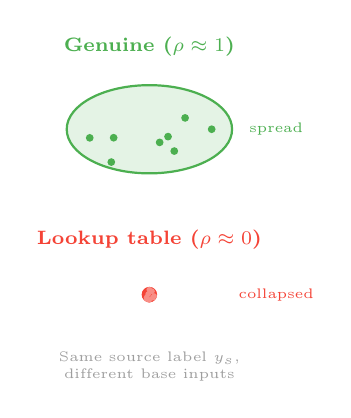
\begin{tikzpicture}[scale=0.7]
  % Genuine intervention
  \node[font=\scriptsize\bfseries,pass] at (0,5.5) {Genuine ($\rho \approx 1$)};
  \fill[pass!15] (0,4.0) ellipse (1.5 and 0.8);
  \draw[pass,thick] (0,4.0) ellipse (1.5 and 0.8);
  \foreach \i in {1,...,8} {
    \pgfmathsetmacro{\x}{1.2*rand}
    \pgfmathsetmacro{\y}{0.6*rand}
    \fill[pass] (\x,4.0+\y) circle (2pt);
  }
  \node[font=\tiny,pass] at (2.3,4.0) {spread};

  % Lookup table
  \node[font=\scriptsize\bfseries,fail] at (0,2.0) {Lookup table ($\rho \approx 0$)};
  \fill[fail] (0,1.0) circle (4pt);
  \foreach \i in {1,...,8} {
    \pgfmathsetmacro{\x}{0.1*rand}
    \pgfmathsetmacro{\y}{0.1*rand}
    \fill[fail!60] (\x,1.0+\y) circle (1.5pt);
  }
  \node[font=\tiny,fail] at (2.3,1.0) {collapsed};

  % Label
  \node[font=\tiny,neutral,align=center] at (0,-0.3) {Same source label $y_s$,\\different base inputs};
\end{tikzpicture}
\end{column}
\end{columns}
\end{frame}

%% --- SLIDE: Four faithfulness metrics ---
\begin{frame}{Four complementary faithfulness metrics}

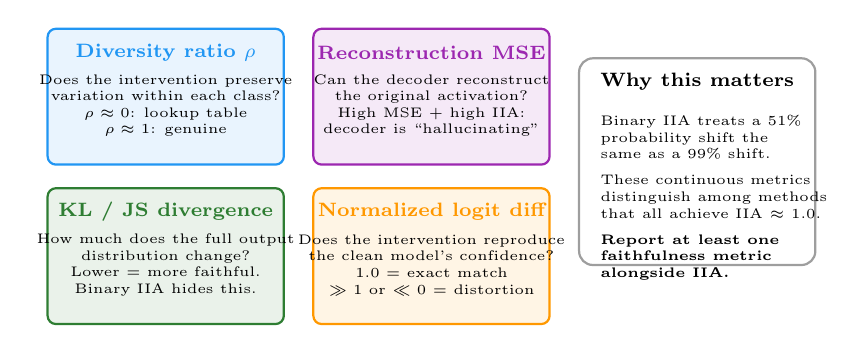
\begin{tikzpicture}[scale=0.75]
  % Metric 1: Diversity ratio
  \fill[das!10,rounded corners=3pt] (-5.5,2.2) rectangle (-1.5,4.5);
  \draw[das,thick,rounded corners=3pt] (-5.5,2.2) rectangle (-1.5,4.5);
  \node[font=\scriptsize\bfseries,das] at (-3.5,4.1) {Diversity ratio $\rho$};
  \node[font=\tiny,align=center] at (-3.5,3.2) {Does the intervention preserve\\variation within each class?\\$\rho \approx 0$: lookup table\\$\rho \approx 1$: genuine};

  % Metric 2: Reconstruction fidelity
  \fill[vae!10,rounded corners=3pt] (-1,2.2) rectangle (3,4.5);
  \draw[vae,thick,rounded corners=3pt] (-1,2.2) rectangle (3,4.5);
  \node[font=\scriptsize\bfseries,vae] at (1,4.1) {Reconstruction MSE};
  \node[font=\tiny,align=center] at (1,3.2) {Can the decoder reconstruct\\the original activation?\\High MSE + high IIA:\\decoder is ``hallucinating''};

  % Metric 3: KL / JS divergence
  \fill[grass!10,rounded corners=3pt] (-5.5,-0.5) rectangle (-1.5,1.8);
  \draw[grass,thick,rounded corners=3pt] (-5.5,-0.5) rectangle (-1.5,1.8);
  \node[font=\scriptsize\bfseries,grass] at (-3.5,1.4) {KL / JS divergence};
  \node[font=\tiny,align=center] at (-3.5,0.5) {How much does the full output\\distribution change?\\Lower = more faithful.\\Binary IIA hides this.};

  % Metric 4: Normalized logit diff
  \fill[nldas!10,rounded corners=3pt] (-1,-0.5) rectangle (3,1.8);
  \draw[nldas,thick,rounded corners=3pt] (-1,-0.5) rectangle (3,1.8);
  \node[font=\scriptsize\bfseries,nldas] at (1,1.4) {Normalized logit diff};
  \node[font=\tiny,align=center] at (1,0.5) {Does the intervention reproduce\\the clean model's confidence?\\1.0 = exact match\\$\gg 1$ or $\ll 0$ = distortion};

  % Why this matters
  \draw[neutral,thick,rounded corners=5pt] (3.5,0.5) rectangle (7.5,4.0);
  \node[font=\scriptsize\bfseries] at (5.5,3.6) {Why this matters};
  \node[font=\tiny,align=left,anchor=north west] at (3.7,3.2) {%
    Binary IIA treats a 51\%\\
    probability shift the\\
    same as a 99\% shift.\\[0.5em]
    These continuous metrics\\
    distinguish among methods\\
    that all achieve IIA $\approx$ 1.0.\\[0.5em]
    \textbf{Report at least one}\\
    \textbf{faithfulness metric}\\
    \textbf{alongside IIA.}};
\end{tikzpicture}
\end{frame}


%% ============================================================
%% PART 4: THE FIX
%% ============================================================

\begin{frame}[plain]
\vfill
\begin{center}
  \setlength{\fboxrule}{2.5pt}%
  \fcolorbox{black}{white}{\parbox{0.7\textwidth}{\centering\vspace{0.8em}
    {\Large\bfseries Part 4}\hypertarget{part4}{}\\[0.5em]
    {\large The fix: structured VAE and cross-task transfer}
  \vspace{0.8em}}}
\end{center}
\vfill
\end{frame}

\begin{frame}{In this section}
\begin{columns}[T]
\begin{column}{0.48\textwidth}
\textbf{\hyperlink{sec10}{10. Structured VAE}}\\[0.2em]
{\small A VAE with causal/nuisance split and ELBO prevents the lookup-table failure. Matches DAS where it works, extends to nonlinear.}

\vspace{0.4em}
\textbf{\hyperlink{sec10b}{10b. Structured pi-SAE (ours)}}\\[0.2em]
{\small Adding L1 sparsity to the label-conditional prior transforms pi-VAE from IIA $= 0$ to IIA $= 1$ on grokked operations. Reveals true intrinsic dimension. CRT composite moduli confirm genuinely 2D causal variables.}

\vspace{0.4em}
\textbf{\hyperlink{sec10c}{10c. NLP tasks}}\\[0.2em]
{\small Structured pi-SAE on GPT-2 language tasks (SVA, greater-than, gender bias, capitals, hypernymy). Detects nonlinear structure that DAS misses.}

\vspace{0.4em}
\textbf{\hyperlink{sec11}{11. Cross-task transfer}}\\[0.2em]
{\small Genuine causal variables transfer across task variants.}
\end{column}
\begin{column}{0.48\textwidth}
\textbf{\hyperlink{sec12}{12. IOI is not Grassmannian}}\\[0.2em]
{\small Sheaf consistency shows IOI's variable is locally linear but globally curved.}

\vspace{0.4em}
\textbf{\hyperlink{sec12b}{From subspaces to factors}}\\[0.2em]
{\small Factorized DAS finds interpretable factor directions within the subspace.}

\vspace{0.4em}
\textbf{\hyperlink{sec12c}{Weight space vs.\ activation space}}\\[0.2em]
{\small Factors decompose how the model computes, not just what it outputs.}
\end{column}
\end{columns}
\end{frame}

\hypertarget{sec10}{}
\section{10. Structured VAE}

%% --- SLIDE: The structured VAE idea ---
\begin{frame}{Structured VAE for nonlinear causal variables}

\begin{columns}[T]
\begin{column}{0.55\textwidth}
{\small The structured VAE partitions the latent space into:}
\begin{itemize}
  \item {\small $z_\text{causal}$: supervised with the operation's label}
  \item {\small $z_\text{nuisance}$: unsupervised, absorbs everything else}
\end{itemize}

\vspace{0.3em}
{\small The loss combines three terms:}
$$\mathcal{L} = \underbrace{-\mathbb{E}_q[\log p(x \mid y, z)]}_{\text{reconstruction}} + \beta \underbrace{D_\text{KL}}_{\text{regularization}} + \alpha \underbrace{\mathcal{L}_\text{CE}}_{\text{supervision}}$$

\vspace{0.3em}
{\small The ELBO prevents the lookup-table failure:}
\begin{enumerate}
  \item {\small Reconstruction forces faithful decoding}
  \item {\small KL prevents latent collapse}
  \item {\small Causal/nuisance split preserves base info}
\end{enumerate}
\end{column}
\begin{column}{0.42\textwidth}
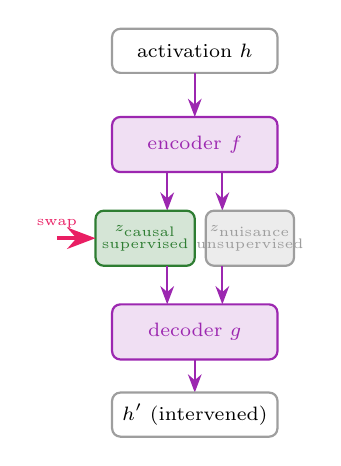
\begin{tikzpicture}[scale=0.7]
  % Input
  \draw[neutral,thick,rounded corners=3pt] (-1.5,5.0) rectangle (1.5,5.8);
  \node[font=\scriptsize] at (0,5.4) {activation $h$};

  % Encoder
  \draw[vae,thick,-{Stealth}] (0,5.0) -- (0,4.2);
  \draw[vae,thick,rounded corners=3pt,fill=vae!15] (-1.5,3.2) rectangle (1.5,4.2);
  \node[font=\scriptsize,vae] at (0,3.7) {encoder $f$};

  % Split
  \draw[vae,thick,-{Stealth}] (-0.5,3.2) -- (-0.5,2.5);
  \draw[vae,thick,-{Stealth}] (0.5,3.2) -- (0.5,2.5);

  % Causal latent
  \fill[grass!20,rounded corners=3pt] (-1.8,1.5) rectangle (0,2.5);
  \draw[grass,thick,rounded corners=3pt] (-1.8,1.5) rectangle (0,2.5);
  \node[font=\tiny,grass,align=center] at (-0.9,2.0) {$z_\text{causal}$\\{\tiny supervised}};

  % Nuisance latent
  \fill[neutral!20,rounded corners=3pt] (0.2,1.5) rectangle (1.8,2.5);
  \draw[neutral,thick,rounded corners=3pt] (0.2,1.5) rectangle (1.8,2.5);
  \node[font=\tiny,neutral,align=center] at (1.0,2.0) {$z_\text{nuisance}$\\{\tiny unsupervised}};

  % Swap arrow
  \draw[circle,ultra thick,-{Stealth}] (-2.5,2.0) -- (-1.8,2.0);
  \node[font=\tiny,circle,above] at (-2.5,2.0) {swap};

  % Decoder
  \draw[vae,thick,-{Stealth}] (-0.5,1.5) -- (-0.5,0.8);
  \draw[vae,thick,-{Stealth}] (0.5,1.5) -- (0.5,0.8);
  \draw[vae,thick,rounded corners=3pt,fill=vae!15] (-1.5,-0.2) rectangle (1.5,0.8);
  \node[font=\scriptsize,vae] at (0,0.3) {decoder $g$};

  % Output
  \draw[vae,thick,-{Stealth}] (0,-0.2) -- (0,-0.8);
  \draw[neutral,thick,rounded corners=3pt] (-1.5,-1.6) rectangle (1.5,-0.8);
  \node[font=\scriptsize] at (0,-1.2) {$h'$ (intervened)};
\end{tikzpicture}
\end{column}
\end{columns}
\end{frame}

%% --- SLIDE: Why VAE is not vacuous ---
\begin{frame}{Why the VAE is not vacuous: three constraints}

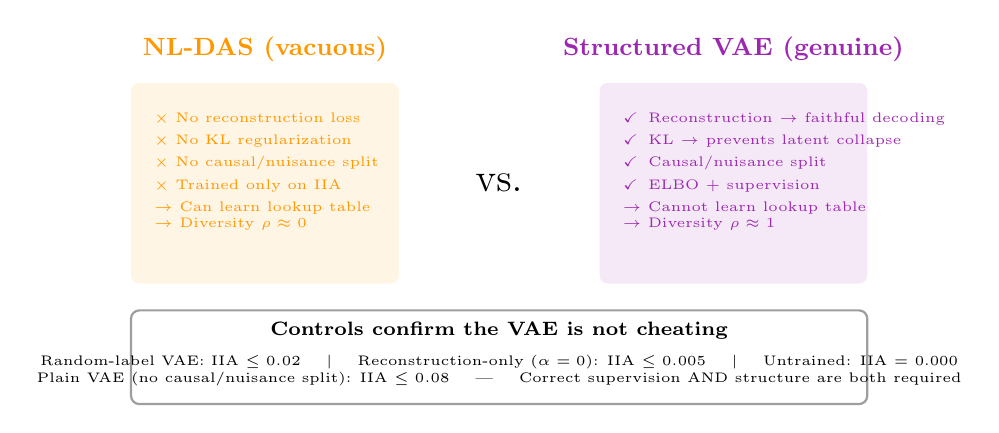
\begin{tikzpicture}[scale=0.85]
  % NL-DAS column
  \node[font=\small\bfseries,nldas] at (-3.5,4.5) {NL-DAS (vacuous)};

  \fill[nldas!10,rounded corners=3pt] (-5.5,1.0) rectangle (-1.5,4.0);
  \node[font=\tiny,nldas,align=left,anchor=north west] at (-5.3,3.7) {%
    $\times$ No reconstruction loss\\[0.3em]
    $\times$ No KL regularization\\[0.3em]
    $\times$ No causal/nuisance split\\[0.3em]
    $\times$ Trained only on IIA\\[0.3em]
    $\to$ Can learn lookup table\\
    $\to$ Diversity $\rho \approx 0$};

  % Arrow
  \node[font=\Large] at (0,2.5) {vs.};

  % VAE column
  \node[font=\small\bfseries,vae] at (3.5,4.5) {Structured VAE (genuine)};

  \fill[vae!10,rounded corners=3pt] (1.5,1.0) rectangle (5.5,4.0);
  \node[font=\tiny,vae,align=left,anchor=north west] at (1.7,3.7) {%
    \checkmark\, Reconstruction $\to$ faithful decoding\\[0.3em]
    \checkmark\, KL $\to$ prevents latent collapse\\[0.3em]
    \checkmark\, Causal/nuisance split\\[0.3em]
    \checkmark\, ELBO + supervision\\[0.3em]
    $\to$ Cannot learn lookup table\\
    $\to$ Diversity $\rho \approx 1$};

  % Controls
  \draw[neutral,thick,rounded corners=3pt] (-5.5,-0.8) rectangle (5.5,0.6);
  \node[font=\scriptsize\bfseries] at (0,0.3) {Controls confirm the VAE is not cheating};
  \node[font=\tiny,align=center] at (0,-0.3) {Random-label VAE: IIA $\leq 0.02$ \quad $|$ \quad Reconstruction-only ($\alpha = 0$): IIA $\leq 0.005$ \quad $|$ \quad Untrained: IIA = 0.000\\
  Plain VAE (no causal/nuisance split): IIA $\leq 0.08$ \quad --- \quad Correct supervision AND structure are both required};
\end{tikzpicture}
\end{frame}

%% --- SLIDE: VAE matches DAS where DAS works ---
\begin{frame}{VAE matches DAS where DAS works, extends where it fails}

\begin{columns}[T]
\begin{column}{0.48\textwidth}
{\small \textbf{Always Grassmannian operations:}\\VAE reduces to an effective rotation.}

\vspace{0.3em}
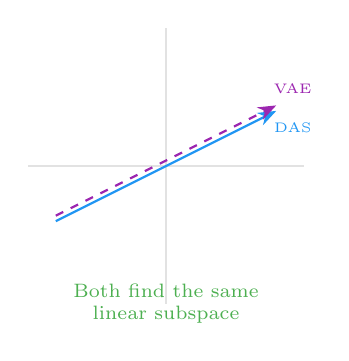
\begin{tikzpicture}[scale=0.7]
  % DAS and VAE agree
  \draw[neutral!30] (-2.5,0) -- (2.5,0);
  \draw[neutral!30] (0,-2.5) -- (0,2.5);

  % Linear subspace
  \draw[das,thick,-{Stealth}] (-2,-1) -- (2,1);
  \draw[vae,thick,dashed,-{Stealth}] (-2,-0.9) -- (2,1.1);

  \node[font=\tiny,das] at (2.3,0.7) {DAS};
  \node[font=\tiny,vae] at (2.3,1.4) {VAE};

  \node[font=\scriptsize,pass,align=center] at (0,-2.5) {Both find the same\\linear subspace};
\end{tikzpicture}
\end{column}
\begin{column}{0.48\textwidth}
{\small \textbf{Never Grassmannian operations:}\\VAE's nonlinear encoder captures curved structure.}

\vspace{0.3em}
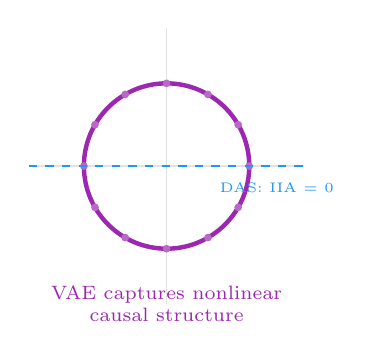
\begin{tikzpicture}[scale=0.7]
  \draw[neutral!30] (-2.5,0) -- (2.5,0);
  \draw[neutral!30] (0,-2.5) -- (0,2.5);

  % Circle
  \draw[vae,ultra thick] (0,0) circle (1.5);
  \foreach \a in {0,30,...,330} {
    \fill[vae!70] ({1.5*cos(\a)},{1.5*sin(\a)}) circle (2pt);
  }

  % DAS fails
  \draw[das,thick,dashed] (-2.5,0) -- (2.5,0);
  \node[font=\tiny,das] at (2.0,-0.4) {DAS: IIA = 0};

  \node[font=\scriptsize,vae,align=center] at (0,-2.5) {VAE captures nonlinear\\causal structure};
\end{tikzpicture}
\end{column}
\end{columns}

\vspace{0.5em}
\centering
{\small For grokked addition and multiplication, both DAS and VAE achieve IIA = 1.000 and equivariance $>99\%$.\\The VAE is a \textbf{strict generalization} of DAS: when the variable is linear, VAE = DAS.}
\end{frame}

\hypertarget{sec10b}{}
\section{10b. Structured pi-SAE: sparse nonlinear causal discovery}

%% --- SLIDE: From VAE to Structured pi-SAE ---
\begin{frame}{From pi-VAE to Structured pi-SAE: sparsity + structure}

\begin{columns}[T]
\begin{column}{0.48\textwidth}
\textbf{pi-VAE} {\small (Zhou \& Wei, 2020)}\\[0.3em]
{\small Label-conditional prior:}
\vspace{-0.2em}
\[ p(z \mid y) = \mathcal{N}\!\bigl(\mu(y),\, \sigma^2(y)\bigr) \]
\vspace{-0.5em}
{\small Instead of the standard $\mathcal{N}(0, I)$ prior, each label gets its own mean and variance. Forces the latent space to organize by label.}

\vspace{0.5em}
{\small Published method. Works well on IOI.}

\vspace{0.3em}
{\small But on grokked modular arithmetic:\\IIA $= 0$ across all $k$.}

\end{column}
\begin{column}{0.48\textwidth}
\textbf{Structured pi-SAE} {\small \textcolor{vae}{(ours)}}\\[0.3em]
{\small pi-VAE + \textbf{causal/nuisance split} + \textbf{L1 sparsity}:}
\vspace{-0.2em}
\[ \mathcal{L} = \mathcal{L}_\text{pi-VAE} + \lambda \|z_c\|_1, \quad z = (z_c, z_n) \]
\vspace{-0.5em}
{\small Explicit causal/nuisance partition forces the model to separate task-relevant from task-irrelevant variation. L1 sparsity on $z_c$ prevents memorization.}

\vspace{0.5em}
{\small \textbf{Our modification.} Results:}

\vspace{0.3em}
\begin{tabular}{@{}lcc@{}}
& \textbf{pi-VAE} & \textbf{Str.\ pi-SAE} \\
\midrule
{\small Addition} & 0.000 & \textbf{\textcolor{always}{1.000}} \\
{\small Multiplication} & 0.000 & \textbf{\textcolor{always}{1.000}} \\
{\small Quartic sum} & 0.000 & \textbf{\textcolor{always}{1.000}} \\
{\small IOI} & 0.945 & \textbf{\textcolor{always}{0.980}} \\
\end{tabular}

\vspace{0.2em}
{\small All at $k{=}2$. Controls $\leq 0.02$.}
\end{column}
\end{columns}

\vspace{0.5em}
\centering
\fcolorbox{vae}{vae!8}{\parbox{0.85\textwidth}{\centering\vspace{0.2em}
{\small Both ingredients matter. pi-VAE (structured prior alone) $\to$ IIA $= 0$. Adding the causal/nuisance split + L1 sparsity transforms it to IIA $= 1$.}
\vspace{0.2em}}}
\end{frame}

%% --- SLIDE: Intrinsic dimension ---
\begin{frame}{Intrinsic dimension: $k{=}1$ reveals the true structure}

\begin{columns}[T]
\begin{column}{0.50\textwidth}
{\small A circle is topologically \textbf{1-dimensional} --- parameterized by a single angle $\theta$.}

\vspace{0.3em}
{\small Linear DAS needs $k{=}2$ because it embeds the circle as $(\cos\theta, \sin\theta)$ on a flat plane.}

\vspace{0.3em}
{\small A nonlinear method can learn $z = \theta$ directly and decode back to the circle. \textbf{Structured pi-SAE at $k{=}1$}:}

\vspace{0.3em}
{\small\setlength{\tabcolsep}{4pt}
\begin{tabular}{@{}lccc@{}}
\toprule
& \textbf{DAS} & \textbf{NL-DAS} & \textbf{Structured pi-SAE} \\
\midrule
Addition & 0.006 & 0.194 & \textbf{\textcolor{always}{0.917}} \\
Multiplication & 0.022 & 0.217 & 0.011 \\
Quartic sum & 0.011 & 0.244 & 0.106 \\
IOI & 0.185 & 1.000 & \textbf{\textcolor{always}{0.988}} \\
\bottomrule
\end{tabular}}

\vspace{0.3em}
{\small Addition's circle admits a smooth 1D parameterization. Multiplication's discrete-log circle does not.}
\end{column}
\begin{column}{0.46\textwidth}
\centering
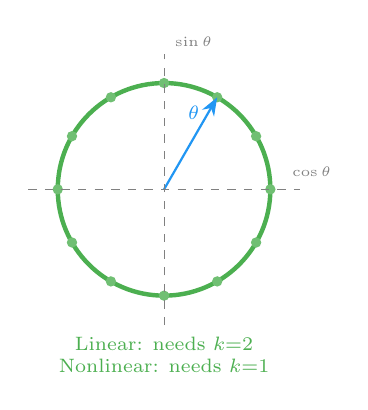
\begin{tikzpicture}[scale=0.75]
  % Circle
  \draw[always,ultra thick] (0,0) circle (1.8);

  % Points on circle
  \foreach \a/\lab in {0/0, 30/1, 60/2, 90/3, 120/4, 150/5, 180/6, 210/7, 240/8, 270/9, 300/10, 330/11} {
    \fill[always!80] ({1.8*cos(\a)},{1.8*sin(\a)}) circle (2.5pt);
  }

  % Angle annotation
  \draw[das,thick,-{Stealth}] (0,0) -- ({1.8*cos(60)},{1.8*sin(60)});
  \node[font=\scriptsize,das] at (0.5,1.3) {$\theta$};

  % k=2 annotation
  \draw[gray,thin,dashed] (-2.3,0) -- (2.3,0);
  \draw[gray,thin,dashed] (0,-2.3) -- (0,2.3);
  \node[font=\tiny,gray] at (2.5,0.3) {$\cos\theta$};
  \node[font=\tiny,gray] at (0.5,2.5) {$\sin\theta$};

  % Labels
  \node[font=\scriptsize,always,align=center] at (0,-2.8) {Linear: needs $k{=}2$\\Nonlinear: needs $k{=}1$};
\end{tikzpicture}

\vspace{0.5em}
\fcolorbox{always}{always!8}{\parbox{0.9\linewidth}{\centering\vspace{0.1em}
  {\small Linear DAS \textbf{overestimates}\\intrinsic dimension.}
\vspace{0.1em}}}
\end{column}
\end{columns}
\end{frame}

%% --- SLIDE: Full results table ---
\begin{frame}{Structured pi-SAE results across all operations}
\vspace{-0.3em}
\centering
{\small\setlength{\tabcolsep}{3pt}
\begin{tabular}{@{}lcccccccc@{}}
\toprule
& & & \multicolumn{3}{c}{\textbf{IIA at $k{=}2$}} & \multicolumn{3}{c}{\textbf{IIA at $k{=}1$}} \\
\cmidrule(lr){4-6} \cmidrule(lr){7-9}
\textbf{Operation} & \textbf{Grok} & \textbf{Acc} & \textbf{DAS} & \textbf{NL-DAS} & \textbf{Str.\ pi-SAE} & \textbf{DAS} & \textbf{NL-DAS} & \textbf{Str.\ pi-SAE} \\
\midrule
Addition & \textcolor{always}{\checkmark} & 1.00 & 0.06 & 0.49 & \textbf{\textcolor{always}{1.00}} & 0.01 & 0.19 & \textbf{\textcolor{always}{0.92}} \\
Multiplication & \textcolor{always}{\checkmark} & 1.00 & 0.08 & 0.72 & \textbf{\textcolor{always}{1.00}} & 0.02 & 0.22 & 0.01 \\
Quartic sum & \textcolor{always}{\checkmark} & 1.00 & 0.03 & 0.79 & \textbf{\textcolor{always}{1.00}} & 0.01 & 0.24 & 0.11 \\
IOI (GPT-2) & --- & --- & 0.30 & \textcolor{never}{1.00} & \textbf{\textcolor{always}{0.98}} & 0.19 & \textcolor{never}{1.00} & \textbf{\textcolor{always}{0.99}} \\
\midrule
Mixed product & \textcolor{never}{$\times$} & 0.15 & 0.02 & \textcolor{never}{0.60} & 0.04 & 0.01 & 0.21 & 0.02 \\
Symmetric power & \textcolor{never}{$\times$} & 0.21 & 0.02 & \textcolor{never}{0.63} & 0.02 & 0.01 & 0.26 & 0.02 \\
Double add mult & \textcolor{never}{$\times$} & 0.10 & 0.00 & \textcolor{never}{0.77} & 0.02 & 0.00 & 0.22 & 0.02 \\
Squaring & \textcolor{never}{$\times$} & 0.01 & 0.00 & 0.01 & 0.00 & 0.00 & 0.01 & 0.00 \\
\bottomrule
\end{tabular}}

\vspace{0.5em}
{\small \textcolor{always}{Green bold}: genuine causal variable found. \textcolor{never}{Red}: NL-DAS vacuity --- high IIA despite no learned structure.}

\vspace{0.3em}
{\small Structured pi-SAE achieves IIA $= 1.0$ on all grokked operations and correctly returns $\approx 0$ on all non-grokked operations. NL-DAS returns 0.6--0.8 on non-grokked operations --- \textbf{false positives}.}
\end{frame}

%% --- SLIDE: The 2x2 ablation ---
\begin{frame}{Ablation: both sparsity and structure are required}
\vspace{-0.2em}
\centering

{\small IIA at $k{=}2$ across the $2 \times 2$ ablation: \{structured prior, plain prior\} $\times$ \{VAE, SAE\}.}

\vspace{0.5em}
{\setlength{\tabcolsep}{4pt}
\begin{tabular}{@{}l|cc|cc@{}}
\toprule
& \multicolumn{2}{c|}{\textbf{Plain prior} $\mathcal{N}(0,I)$} & \multicolumn{2}{c}{\textbf{Structured prior} $p(z|y)$} \\
\textbf{Operation} & VAE & SAE & pi-VAE & \textbf{Str.\ pi-SAE} \\
\midrule
Addition & 0.02 & \textcolor{always}{1.00} & 0.00 & \textbf{\textcolor{always}{1.00}} \\
Multiplication & 0.00 & 0.72 & 0.00 & \textbf{\textcolor{always}{1.00}} \\
Quartic sum & 0.02 & 0.32 & 0.00 & \textbf{\textcolor{always}{1.00}} \\
IOI & 0.56 & 0.83 & \textcolor{always}{0.95} & \textbf{\textcolor{always}{0.98}} \\
\midrule
Mixed product & 0.03 & 0.01 & 0.01 & 0.04 \\
Squaring & 0.00 & 0.00 & 0.00 & 0.00 \\
\bottomrule
\end{tabular}}

\vspace{0.5em}
\begin{columns}[T]
\begin{column}{0.48\textwidth}
\fcolorbox{never}{never!8}{\parbox{0.9\linewidth}{\centering\vspace{0.15em}
  {\small \textbf{Plain SAE} works on addition\\but degrades on multiplication\\and quartic sum.}
\vspace{0.15em}}}
\end{column}
\begin{column}{0.48\textwidth}
\fcolorbox{always}{always!8}{\parbox{0.9\linewidth}{\centering\vspace{0.15em}
  {\small \textbf{Structured pi-SAE} is uniformly best.\\Structured prior + sparsity\\= robust across all tasks.}
\vspace{0.15em}}}
\end{column}
\end{columns}

\vspace{0.3em}
\centering
{\small Neither component alone suffices: pi-VAE (no sparsity, no split) $= 0$; SAE (no structured prior) is inconsistent. Only Structured pi-SAE (prior + split + sparsity) works uniformly.}
\end{frame}

%% --- SLIDE: NL-DAS vacuity exposed ---
\begin{frame}{Structured pi-SAE exposes NL-DAS vacuity}

\begin{columns}[T]
\begin{column}{0.48\textwidth}
\textbf{The problem:}\\[0.3em]
{\small NL-DAS achieves IIA $= 0.6$--$0.8$ on operations that \textbf{never learned} the task (test accuracy $< 20\%$).}

\vspace{0.3em}
{\small These are false positives. The encoder--decoder learned a lookup table, not a causal variable.}

\vspace{0.5em}
\textbf{Structured pi-SAE correctly rejects:}\\[0.3em]
{\small On the same operations, Structured pi-SAE returns IIA $\leq 0.04$. The reconstruction constraint prevents hallucination.}

\vspace{0.3em}
{\small Reconstruction MSE confirms:}\\[0.2em]
{\small\setlength{\tabcolsep}{3pt}
\begin{tabular}{@{}lcc@{}}
& \textbf{Grokked} & \textbf{Not grokked} \\
\midrule
{\small Recon MSE} & 0.6--1.2 & 11--24 \\
{\small Classifier acc} & 1.00 & 0.06--0.63 \\
\end{tabular}}
\end{column}
\begin{column}{0.48\textwidth}
\centering
\vspace{0.5em}
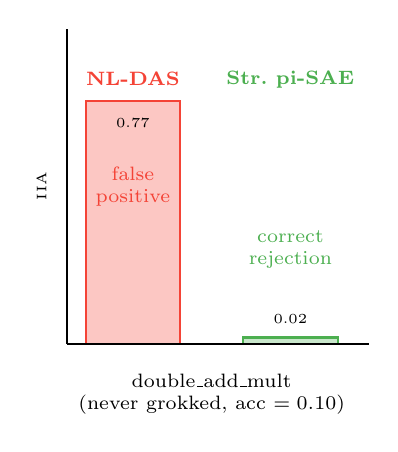
\begin{tikzpicture}[scale=0.8]
  % NL-DAS bar
  \fill[never!30] (0,0) rectangle (1.5,3.85);
  \draw[never,thick] (0,0) rectangle (1.5,3.85);
  \node[font=\scriptsize\bfseries,never] at (0.75,4.2) {NL-DAS};
  \node[font=\tiny] at (0.75,3.5) {0.77};

  % Structured pi-SAE bar
  \fill[always!30] (2.5,0) rectangle (4.0,0.1);
  \draw[always,thick] (2.5,0) rectangle (4.0,0.1);
  \node[font=\scriptsize\bfseries,always] at (3.25,4.2) {Str.\ pi-SAE};
  \node[font=\tiny] at (3.25,0.4) {0.02};

  % Axis
  \draw[thick] (-0.3,0) -- (4.5,0);
  \draw[thick] (-0.3,0) -- (-0.3,5);
  \node[font=\tiny,rotate=90] at (-0.7,2.5) {IIA};
  \node[font=\scriptsize,align=center] at (2.0,-0.8) {double\_add\_mult\\(never grokked, acc $= 0.10$)};

  % Verdict
  \node[font=\scriptsize,never,align=center] at (0.75,2.5) {false\\positive};
  \node[font=\scriptsize,always,align=center] at (3.25,1.5) {correct\\rejection};
\end{tikzpicture}
\end{column}
\end{columns}

\vspace{0.3em}
\centering
\fcolorbox{vae}{vae!8}{\parbox{0.85\textwidth}{\centering\vspace{0.1em}
{\small \textbf{Recommendation}: replace NL-DAS with Structured pi-SAE for nonlinear causal discovery. Same expressivity, no vacuity.}
\vspace{0.1em}}}
\end{frame}

%% --- SLIDE: CRT composite modulus ---
\begin{frame}{CRT composite modulus: the first task needing $k{>}1$}
\begin{columns}[T]
\begin{column}{0.48\textwidth}
\textbf{Chinese Remainder Theorem.}\\[0.3em]
For composite modulus $n = p \times q$:
\[ \mathbb{Z}/n\mathbb{Z} \;\cong\; \mathbb{Z}/p\mathbb{Z} \times \mathbb{Z}/q\mathbb{Z} \]
The model learns \textbf{two independent circles} ---
one mod $p$, one mod $q$.\\[0.3em]

{\small
Intrinsic dimension = \textbf{2} (two angles $\theta_p, \theta_q$).\\
Linear DAS needs $k \geq 4$ ($\cos/\sin$ for each).\\
Structured pi-SAE captures both at $k{=}2$.}\\[0.5em]

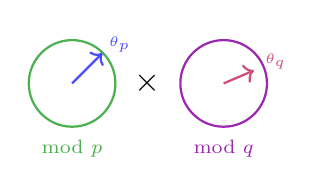
\begin{tikzpicture}[scale=0.55]
  \draw[always,thick] (0,0) circle (1.0);
  \node[font=\scriptsize,always] at (0,-1.5) {mod $p$};
  \draw[->,thick,blue!70] (0,0) -- (0.7,0.7);
  \node[font=\tiny,blue!70] at (1.1,0.9) {$\theta_p$};
  \draw[vae,thick] (3.5,0) circle (1.0);
  \node[font=\scriptsize,vae] at (3.5,-1.5) {mod $q$};
  \draw[->,thick,purple!70] (3.5,0) -- (4.2,0.3);
  \node[font=\tiny,purple!70] at (4.7,0.5) {$\theta_q$};
  \node[font=\large] at (1.75,0) {$\times$};
\end{tikzpicture}
\end{column}
\begin{column}{0.52\textwidth}
{\scriptsize
\begin{tabular}{@{}lcrrrl@{}}
\toprule
\textbf{Task} & $k$ & \textbf{DAS} & \textbf{NL-D} & \textbf{Str.\ pi-SAE} & \\
\midrule
add 113 & 1 & 0.01 & 0.19 & \textcolor{always}{\textbf{0.92}} & {\color{always}\checkmark} \\
(prime) & 2 & 0.06 & 0.49 & \textcolor{always}{\textbf{1.00}} & \\[0.2em]
add mod 77 & 1 & 0.02 & 0.19 & 0.06 & {\color{always}\checkmark} \\
($7 \times 11$) & 2 & 0.07 & 0.59 & \textcolor{always}{\textbf{0.99}} & \\[0.2em]
add mod 91 & 1 & 0.02 & 0.24 & 0.00 & {\color{always}\checkmark} \\
($7 \times 13$) & 2 & 0.16 & 0.70 & \textcolor{always}{\textbf{0.98}} & \\[0.2em]
add mod 35 & 2 & 0.08 & \textcolor{never}{\textbf{0.51}} & 0.21 & {\color{never}$\times$} \\
($5 \times 7$) & 4 & 0.21 & \textcolor{never}{\textbf{0.95}} & 0.21 & \\
\bottomrule
\end{tabular}
}\\[0.3em]

{\scriptsize
\textcolor{always}{\textbf{Green}}: genuine. \textcolor{never}{\textbf{Red}}: NL-DAS false positive.\\[0.2em]
$k{=}1$ fails on CRT tasks $\Rightarrow$ intrinsic dim is truly 2.\\
Structured pi-SAE $k{=}2$ beats DAS $k{=}8$ (0.86--0.89).
}
\end{column}
\end{columns}
\end{frame}

%% --- SLIDE: CRT k-sweep ---
\begin{frame}{CRT $k$-sweep: linear DAS needs $4\times$ more dimensions}

{\small Addition mod 91 ($= 7 \times 13$). Full $k$-sweep from 1 to 8:}

\vspace{0.3em}
{\small
\begin{tabular}{@{}crrrrrr@{}}
\toprule
& \multicolumn{6}{c}{\textbf{IIA at each $k$}} \\
\cmidrule(l){2-7}
\textbf{Method} & $k{=}1$ & $k{=}2$ & $k{=}3$ & $k{=}4$ & $k{=}6$ & $k{=}8$ \\
\midrule
DAS (linear) & 0.02 & 0.16 & 0.27 & 0.56 & 0.78 & 0.86 \\
NL-DAS & 0.24 & \textcolor{never}{\textbf{0.70}} & \textcolor{never}{\textbf{0.94}} & \textcolor{never}{\textbf{0.92}} & \textcolor{never}{\textbf{0.92}} & \textcolor{never}{\textbf{0.88}} \\
Str.\ pi-SAE (ours) & 0.00 & \textcolor{always}{\textbf{0.98}} & \textcolor{always}{\textbf{0.98}} & \textcolor{always}{\textbf{0.98}} & \textcolor{always}{\textbf{0.98}} & \textcolor{always}{\textbf{0.98}} \\
\bottomrule
\end{tabular}
}

\vspace{0.5em}
\begin{columns}[T]
\begin{column}{0.48\textwidth}
\centering
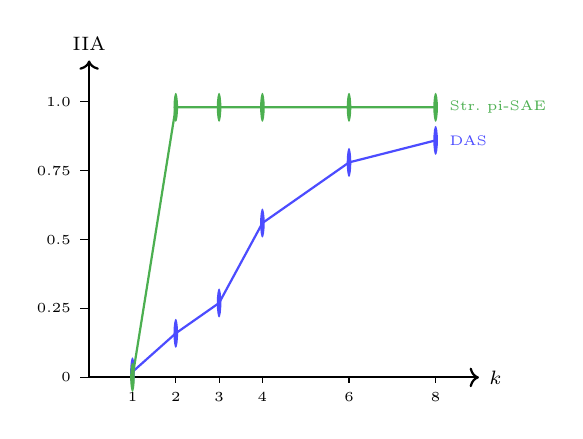
\begin{tikzpicture}[xscale=0.55,yscale=3.5]
  % Axes
  \draw[thick,->] (0,0) -- (9,0) node[right,font=\scriptsize] {$k$};
  \draw[thick,->] (0,0) -- (0,1.15) node[above,font=\scriptsize] {IIA};
  % Y ticks
  \foreach \y/\l in {0.0/0, 0.25/0.25, 0.5/0.5, 0.75/0.75, 1.0/1.0}
    \draw (0,\y) -- (-0.2,\y) node[left,font=\tiny] {\l};
  % X ticks
  \foreach \x in {1,2,3,4,6,8}
    \draw (\x,0) -- (\x,-0.02) node[below,font=\tiny] {\x};
  % DAS line
  \draw[blue!70,thick] (1,0.02) -- (2,0.16) -- (3,0.27) -- (4,0.56) -- (6,0.78) -- (8,0.86);
  \foreach \x/\y in {1/0.02,2/0.16,3/0.27,4/0.56,6/0.78,8/0.86}
    \fill[blue!70] (\x,\y) circle (1.5pt);
  % Structured pi-SAE line
  \draw[always,thick] (1,0.0) -- (2,0.98) -- (3,0.98) -- (4,0.98) -- (6,0.98) -- (8,0.98);
  \foreach \x/\y in {1/0.0,2/0.98,3/0.98,4/0.98,6/0.98,8/0.98}
    \fill[always] (\x,\y) circle (1.5pt);
  % Labels
  \node[font=\tiny,blue!70,right] at (8.1,0.86) {DAS};
  \node[font=\tiny,always,right] at (8.1,0.98) {Str.\ pi-SAE};
\end{tikzpicture}

{\scriptsize Addition mod 91 ($7 \times 13$)}
\end{column}
\begin{column}{0.48\textwidth}
\centering
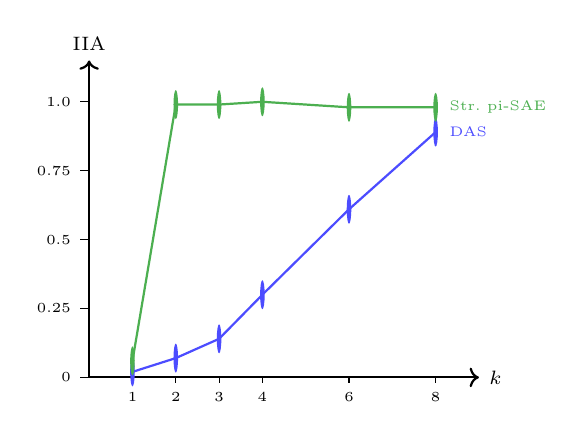
\begin{tikzpicture}[xscale=0.55,yscale=3.5]
  % Axes
  \draw[thick,->] (0,0) -- (9,0) node[right,font=\scriptsize] {$k$};
  \draw[thick,->] (0,0) -- (0,1.15) node[above,font=\scriptsize] {IIA};
  % Y ticks
  \foreach \y/\l in {0.0/0, 0.25/0.25, 0.5/0.5, 0.75/0.75, 1.0/1.0}
    \draw (0,\y) -- (-0.2,\y) node[left,font=\tiny] {\l};
  % X ticks
  \foreach \x in {1,2,3,4,6,8}
    \draw (\x,0) -- (\x,-0.02) node[below,font=\tiny] {\x};
  % DAS line (mod 77)
  \draw[blue!70,thick] (1,0.02) -- (2,0.07) -- (3,0.14) -- (4,0.30) -- (6,0.61) -- (8,0.89);
  \foreach \x/\y in {1/0.02,2/0.07,3/0.14,4/0.30,6/0.61,8/0.89}
    \fill[blue!70] (\x,\y) circle (1.5pt);
  % Structured pi-SAE line (mod 77)
  \draw[always,thick] (1,0.06) -- (2,0.99) -- (3,0.99) -- (4,1.0) -- (6,0.98) -- (8,0.98);
  \foreach \x/\y in {1/0.06,2/0.99,3/0.99,4/1.0,6/0.98,8/0.98}
    \fill[always] (\x,\y) circle (1.5pt);
  % Labels
  \node[font=\tiny,blue!70,right] at (8.1,0.89) {DAS};
  \node[font=\tiny,always,right] at (8.1,0.98) {Str.\ pi-SAE};
\end{tikzpicture}

{\scriptsize Addition mod 77 ($7 \times 11$)}
\end{column}
\end{columns}

\vspace{0.3em}
\centering
{\small Structured pi-SAE saturates at $k{=}2$ (intrinsic dimension). DAS climbs linearly --- still hasn't converged at $k{=}8$.}
\end{frame}

%% --- SLIDE: CRT dimension hierarchy ---
\begin{frame}{Intrinsic dimension hierarchy: prime vs.\ composite}

\begin{columns}[T]
\begin{column}{0.55\textwidth}
{\small The minimum $k$ at which Structured pi-SAE achieves IIA $\geq 0.9$ reveals the \textbf{true intrinsic dimension} of the causal variable:}

\vspace{0.5em}
\begin{tabular}{@{}llcl@{}}
\toprule
\textbf{Operation} & \textbf{Structure} & \textbf{Min $k$} & \textbf{Manifold} \\
\midrule
add mod 113 & prime & 1 & $S^1$ \\
add mod 77 & $7 \times 11$ & 2 & $S^1 \times S^1$ \\
add mod 91 & $7 \times 13$ & 2 & $S^1 \times S^1$ \\
IOI (GPT-2) & NLP & 1 & $S^1$? \\
\bottomrule
\end{tabular}

\vspace{0.5em}
{\small\textbf{Prediction}: addition mod $p_1 \cdots p_n$ needs $k = n$.\\
Testable: mod $2310 = 2{\times}3{\times}5{\times}7{\times}11$ would need $k{=}5$.}

\vspace{0.5em}
{\small Linear DAS always overestimates:}\\[0.2em]
{\footnotesize
\begin{tabular}{@{}lcc@{}}
& \textbf{Linear $k$} & \textbf{Nonlinear $k$} \\
\midrule
Prime ($S^1$) & 2 & \textbf{1} \\
Composite ($S^1 {\times} S^1$) & 4+ & \textbf{2} \\
\end{tabular}
}
\end{column}
\begin{column}{0.42\textwidth}
\centering

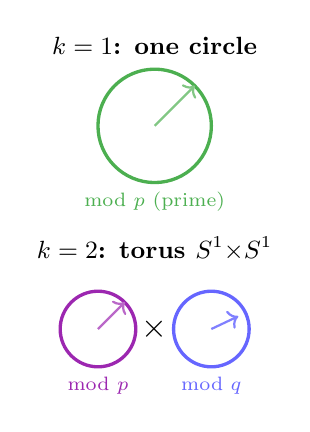
\begin{tikzpicture}[scale=0.6]
  % Level 1: single circle
  \node[font=\small\bfseries] at (2,6.5) {$k=1$: one circle};
  \draw[always,very thick] (2,4.8) circle (1.2);
  \node[font=\scriptsize,always] at (2,3.2) {mod $p$ (prime)};
  \draw[->,thick,always!70] (2,4.8) -- (2.85,5.65);

  % Level 2: torus (two circles)
  \node[font=\small\bfseries] at (2,2.2) {$k=2$: torus $S^1 {\times} S^1$};

  % Draw torus as two linked circles
  \draw[vae,very thick] (0.8,0.5) circle (0.8);
  \draw[blue!60,very thick] (3.2,0.5) circle (0.8);
  \node[font=\scriptsize,vae] at (0.8,-0.7) {mod $p$};
  \node[font=\scriptsize,blue!60] at (3.2,-0.7) {mod $q$};
  \draw[->,thick,vae!70] (0.8,0.5) -- (1.37,1.07);
  \draw[->,thick,blue!50] (3.2,0.5) -- (3.77,0.77);
  \node[font=\large] at (2,0.5) {$\times$};
\end{tikzpicture}

\vspace{0.3em}
{\scriptsize Nonlinear methods reveal the manifold's true topology, not its linear embedding dimension.}
\end{column}
\end{columns}
\end{frame}

%% ===================================================================
%% 10c. NLP tasks: Structured pi-SAE on GPT-2 language tasks
%% ===================================================================
\hypertarget{sec10c}{}
\section{10c. Beyond grokking: NLP tasks on GPT-2}

%% --- SLIDE: NLP task results overview ---
\begin{frame}{Structured pi-SAE on GPT-2 language tasks}

\begin{columns}[T]
\begin{column}{0.55\textwidth}
{\small Beyond toy grokking models: apply Structured pi-SAE to \textbf{real NLP tasks} in GPT-2-small at layer 10.}

\vspace{0.3em}
{\small Using MIB counterfactual pairs (Hanna et al.\ 2024):}
\begin{itemize}
  \item {\small \textbf{SVA}: singular/plural agreement (12,400 pairs)}
  \item {\small \textbf{Greater-than}: year comparison (1,000 pairs)}
  \item {\small \textbf{Gender bias}: occupation $\to$ he/she (986 pairs)}
  \item {\small \textbf{Capitals}: country $\to$ capital (190 pairs)}
  \item {\small \textbf{Hypernymy}: word $\to$ category (198 pairs)}
\end{itemize}

\vspace{0.3em}
{\small Key question: does Structured pi-SAE's \textbf{conservatism} --- only reporting high IIA when genuine low-dimensional structure exists --- hold on language tasks?}
\end{column}
\begin{column}{0.44\textwidth}
{\scriptsize\centering
\renewcommand{\arraystretch}{1.15}
\begin{tabular}{l|ccc}
\toprule
\textbf{Task} & \textbf{DAS} & \textbf{NL-DAS} & \textbf{Str.\ pi-SAE} \\
\midrule
\multicolumn{4}{c}{\textit{$k = 1$}} \\
\midrule
SVA        & 0.00 & \textcolor{red}{1.00} & 0.00 \\
Greater-th & 0.03 & \textcolor{red}{1.00} & 0.00 \\
Gender bias& 0.88 & \textcolor{red}{1.00} & 0.54 \\
Capitals   & 0.00 & 0.00 & \textbf{0.12} \\
Hypernymy  & 0.03 & 0.20 & \textbf{0.50} \\
\midrule
\multicolumn{4}{c}{\textit{$k = 4$}} \\
\midrule
SVA        & 0.02 & \textcolor{red}{1.00} & 0.00 \\
Greater-th & 0.31 & \textcolor{red}{1.00} & 0.00 \\
Gender bias& \textbf{1.00} & \textcolor{red}{1.00} & 0.95 \\
Capitals   & 0.02 & 0.07 & \textbf{0.37} \\
Hypernymy  & 0.08 & 0.43 & \textbf{0.47} \\
\bottomrule
\end{tabular}
}

\vspace{0.3em}
{\scriptsize \textcolor{red}{Red}: NL-DAS false positives (IIA $\approx 1$ on tasks where linear DAS $\approx 0$).}
\end{column}
\end{columns}
\end{frame}

%% --- SLIDE: NLP interpretation ---
\begin{frame}{Interpretation: Structured pi-SAE as a causal structure detector}

\begin{columns}[T]
\begin{column}{0.50\textwidth}
\textbf{Three regimes:}

\vspace{0.3em}
{\small \textbf{1. High-dimensional tasks} (SVA, greater-than):}\\
{\small $\bullet$ All methods except NL-DAS get $\approx 0$\\
$\bullet$ NL-DAS gets $\approx 1.0$ = \textcolor{red}{false positive}\\
$\bullet$ Structured pi-SAE correctly returns 0 --- no low-dim structure}

\vspace{0.3em}
{\small \textbf{2. Genuinely low-dim} (gender bias):}\\
{\small $\bullet$ Binary task (he/she), well-represented linearly\\
$\bullet$ DAS gets 0.88--1.0, Structured pi-SAE gets 0.54--0.95\\
$\bullet$ Structured pi-SAE recovers but needs $k \geq 2$}

\vspace{0.3em}
{\small \textbf{3. Nonlinear structure} (capitals, hypernymy):}\\
{\small $\bullet$ DAS fails ($\approx 0$), NL-DAS also weak\\
$\bullet$ \textbf{Structured pi-SAE is the only method that finds structure}\\
$\bullet$ Capitals: 0.40 at $k{=}2$; hypernymy: 0.50 at $k{=}1$}
\end{column}
\begin{column}{0.48\textwidth}

\vspace{0.5em}
\textbf{Comparison with factorized DAS}\\[0.3em]
{\scriptsize Hard-mode IIA, layer 8, $k{=}1$, atomic-sweep-40:}

\vspace{0.2em}
{\scriptsize\centering
\renewcommand{\arraystretch}{1.15}
\begin{tabular}{l|cc}
\toprule
\textbf{Task} & \textbf{DAS} & \textbf{Fac.\ DAS} \\
\midrule
IOI       & 0.94 & 0.94 \\
SVA       & 0.79 & 0.79 \\
Gender    & 0.79 & 0.83 \\
Capitals  & 0.69 & 0.69 \\
Hypernymy & 1.00 & 1.00 \\
\bottomrule
\end{tabular}
}

\vspace{0.5em}
{\scriptsize Factorized DAS matches optimal DAS exactly.\\[0.2em]
Structured pi-SAE complements: it \textbf{detects} nonlinear structure that DAS misses (capitals, hypernymy), but DAS has higher IIA on linearly-accessible variables (gender bias).\\[0.2em]
\textbf{Together}: structure detection (Structured pi-SAE) + subspace identification (factorized DAS).}
\end{column}
\end{columns}
\end{frame}

\hypertarget{sec11}{}
\section{11. Cross-task transfer}

%% --- SLIDE: Cross-task transfer on IOI ---
\begin{frame}{Cross-task transfer validates causal variables}

\begin{columns}[T]
\begin{column}{0.55\textwidth}
{\small A genuine causal variable should \textbf{transfer} --- train on one task variant, test on another.}

\vspace{0.3em}
{\small \textbf{IOI cross-template transfer} (GPT-2):}
\begin{itemize}
  \item {\small Train VAE on templates 1--3}
  \item {\small Test on unseen templates 4--5}
  \item {\small IIA = 0.82--0.96 at $k = 4$}
\end{itemize}

\vspace{0.3em}
{\small \textbf{Extended IOI tasks}\footnote{\tiny Nainani et al., arXiv:2411.16105, 2024.}:}
\begin{itemize}
  \item {\small DoubleIO: IIA = 0.77--0.81}
  \item {\small TripleIO: IIA = 0.77--0.81}
  \item {\small Trained only on base IOI!}
\end{itemize}

\vspace{0.3em}
{\small \textbf{IOI subtask transfer}\footnote{\tiny Prakash et al., ``Fine-Tuning Enhances Existing Mechanisms,'' ICLR 2024 (MIB benchmark).} (8 counterfactual types):}
\begin{itemize}
  \item {\small DAS transfer ratio: 0.56}
  \item {\small VAE transfer ratio: 0.43}
\end{itemize}
\end{column}
\begin{column}{0.42\textwidth}
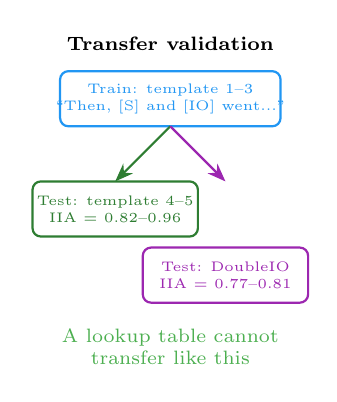
\begin{tikzpicture}[scale=0.7]
  % Transfer diagram
  \node[font=\scriptsize\bfseries] at (0,5.0) {Transfer validation};

  % Train
  \draw[das,thick,rounded corners=3pt] (-2,3.5) rectangle (2,4.5);
  \node[font=\tiny,das,align=center] at (0,4.0) {Train: template 1--3\\``Then, [S] and [IO] went...''};

  % Test 1
  \draw[grass,thick,-{Stealth}] (0,3.5) -- (-1,2.5);
  \draw[grass,thick,rounded corners=3pt] (-2.5,1.5) rectangle (0.5,2.5);
  \node[font=\tiny,grass,align=center] at (-1,2.0) {Test: template 4--5\\IIA = 0.82--0.96};

  % Test 2
  \draw[vae,thick,-{Stealth}] (0,3.5) -- (1,2.5);
  \draw[vae,thick,rounded corners=3pt] (-0.5,0.3) rectangle (2.5,1.3);
  \node[font=\tiny,vae,align=center] at (1,0.8) {Test: DoubleIO\\IIA = 0.77--0.81};

  % The point
  \node[font=\scriptsize,pass,align=center] at (0,-0.5) {A lookup table cannot\\transfer like this};
\end{tikzpicture}
\end{column}
\end{columns}
\end{frame}

\hypertarget{sec12}{}
\section{12. IOI is not Grassmannian}

%% --- SLIDE: Sheaf consistency ---
\begin{frame}{IOI is NOT Grassmannian: sheaf consistency analysis}

\begin{columns}[T]
\begin{column}{0.55\textwidth}
{\small Even within GPT-2's IOI circuit, the causal variable is not globally linear.}

\vspace{0.3em}
{\small We fit local DAS subspaces to different clusters of activations and measure consistency:}

\vspace{0.3em}
\begin{itemize}
  \item {\small Geodesic distance between local subspaces: \textbf{$\sim$2.2}}
  \item {\small Cross-cluster IIA: \textbf{$\sim$0.21}}
\end{itemize}

\vspace{0.3em}
{\small If IOI were Grassmannian, local subspaces would agree (geodesic $\approx 0$, cross-IIA $\approx 1.0$).}

\vspace{0.3em}
{\small The subspace that represents the indirect object \textbf{rotates} across different activation clusters. Locally linear, globally nonlinear --- like a curved manifold approximated by tangent planes.}

\vspace{0.3em}
{\small This is why the VAE outperforms DAS on IOI at $k = 4$ (IIA 0.978 vs.\ 0.556).}
\end{column}
\begin{column}{0.42\textwidth}
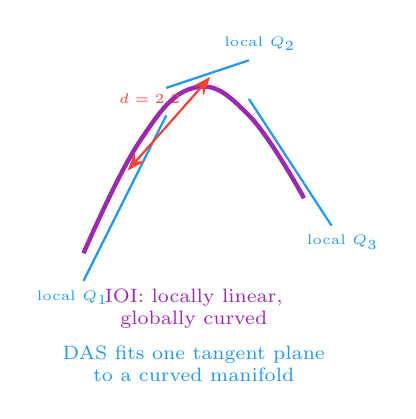
\begin{tikzpicture}[scale=0.7]
  % Curved manifold
  \draw[vae,ultra thick] plot[smooth,tension=0.7]
    coordinates {(-2,-1) (-1,1) (0,2) (1,1.5) (2,0)};

  % Local tangent planes
  \draw[das,thick] (-2.0,-1.5) -- (-0.5,1.5);
  \node[font=\tiny,das] at (-2.2,-1.8) {local $Q_1$};

  \draw[das,thick] (-0.5,2.0) -- (1.0,2.5);
  \node[font=\tiny,das] at (1.2,2.8) {local $Q_2$};

  \draw[das,thick] (1.0,1.8) -- (2.5,-0.5);
  \node[font=\tiny,das] at (2.7,-0.8) {local $Q_3$};

  % Geodesic distances
  \draw[never,thick,{Stealth}-{Stealth}] (-1.2,0.5) -- (0.3,2.2);
  \node[font=\tiny,never] at (-0.8,1.8) {$d = 2.2$};

  % Label
  \node[font=\scriptsize,vae,align=center] at (0,-2.0) {IOI: locally linear,\\globally curved};
  \node[font=\scriptsize,das,align=center] at (0,-3.0) {DAS fits one tangent plane\\to a curved manifold};
\end{tikzpicture}
\end{column}
\end{columns}
\end{frame}


%% --- SLIDE: From subspaces to factors ---
\hypertarget{sec12b}{}
\begin{frame}{From subspaces to interpretable factors}
\vspace{-0.3em}
\begin{columns}[T]
\begin{column}{0.52\textwidth}
{\small DAS finds a subspace. But which \emph{directions} compose it?}

\vspace{0.2em}
{\small If the model's weight matrices decompose as $W_i = S_i \cdot F$ through a shared \textbf{factor bank} $F$ with sparse \textbf{selectors} $S_i$, then DAS can be constrained to search within the factor span:}

\vspace{0.2em}
\begin{tabular}{@{}l@{~}l@{}}
\textbf{\small Standard DAS:} & {\small $U = \mathrm{orth}(A)$, $A \in \R^{d_m \times k}$}\\
\textbf{\small Factorized DAS:} & {\small $U = \mathrm{orth}(F^\top A)$, $A \in \R^{N_F \times k}$}\\
\end{tabular}

\vspace{0.2em}
{\small With a group lasso penalty ($\lambda \sum_i \|A_{i,:}\|_2$), most factors are killed. What survives is interpretable:}

\vspace{0.2em}
{\small\setlength{\tabcolsep}{3pt}
\begin{tabular}{lccl}
\toprule
\textbf{Task} & \textbf{Active} & \textbf{Total} & \textbf{Top factor decodes to} \\
\midrule
IOI & 9 & 1024 & \emph{wives, women, Ms} \\
Gender bias & 3 & 1024 & \emph{she, her, herself} \\
SVA & 2 & 1024 & \emph{are, is, aren't} \\
\bottomrule
\end{tabular}}
\end{column}
\begin{column}{0.44\textwidth}
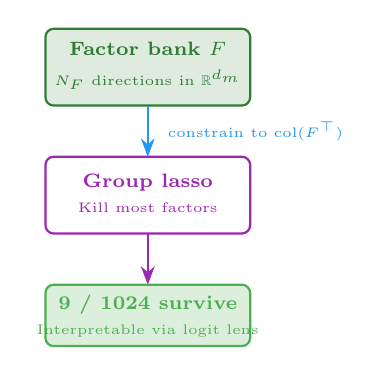
\begin{tikzpicture}[scale=0.65]
  % Factor bank
  \fill[grass!15,rounded corners=3pt] (-0.5,4.5) rectangle (3.5,6.0);
  \draw[grass,thick,rounded corners=3pt] (-0.5,4.5) rectangle (3.5,6.0);
  \node[font=\scriptsize\bfseries,grass] at (1.5,5.6) {Factor bank $F$};
  \node[font=\tiny,grass] at (1.5,5.0) {$N_F$ directions in $\R^{d_m}$};

  % DAS search
  \draw[das,thick,-{Stealth}] (1.5,4.5) -- (1.5,3.5);
  \node[font=\tiny,das,right] at (1.7,4.0) {constrain to $\mathrm{col}(F^\top)$};

  % Group lasso
  \draw[vae,thick,rounded corners=3pt] (-0.5,2.0) rectangle (3.5,3.5);
  \node[font=\scriptsize\bfseries,vae] at (1.5,3.0) {Group lasso};
  \node[font=\tiny,vae] at (1.5,2.5) {Kill most factors};

  % Surviving factors
  \draw[vae,thick,-{Stealth}] (1.5,2.0) -- (1.5,1.0);

  \fill[always!20,rounded corners=3pt] (-0.5,-0.2) rectangle (3.5,1.0);
  \draw[always,thick,rounded corners=3pt] (-0.5,-0.2) rectangle (3.5,1.0);
  \node[font=\scriptsize\bfseries,always] at (1.5,0.6) {9 / 1024 survive};
  \node[font=\tiny,always] at (1.5,0.1) {Interpretable via logit lens};
\end{tikzpicture}

\vspace{0.3em}
\fcolorbox{das}{das!10}{\parbox{0.9\linewidth}{\centering\vspace{0.1em}
  {\small Standard DAS finds the subspace.\\Factorized DAS finds the \textbf{factors} in it.}
\vspace{0.1em}}}
\end{column}
\end{columns}

\vspace{0.1em}
{\footnotesize Results from GPT-2 with sparse weight factorization (Tower, Vegner, Siddharth \& Doumas, in preparation).}
\end{frame}


%% --- SLIDE: Weight space vs activation space ---
\hypertarget{sec12c}{}
\begin{frame}{Weight space vs.\ activation space}

{\small Both SAEs and sparse weight factorization produce dictionaries of directions in the residual stream. But they decompose different things:}

\vspace{0.5em}
\begin{columns}[T]
\begin{column}{0.48\textwidth}
\centering
\textbf{\textcolor{nldas}{SAEs (activation space)}}%
\footnote{\tiny Cunningham et al., ``Sparse Autoencoders Find Highly Interpretable Directions,'' ICLR 2024.}

\vspace{0.3em}
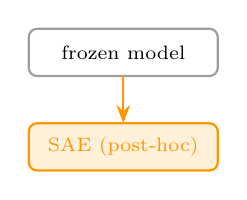
\begin{tikzpicture}[scale=0.6]
  \draw[neutral,thick,rounded corners=3pt] (-2,2) rectangle (2,3);
  \node[font=\scriptsize] at (0,2.5) {frozen model};
  \draw[nldas,thick,-{Stealth}] (0,2) -- (0,1);
  \draw[nldas,thick,rounded corners=3pt,fill=nldas!15] (-2,0) rectangle (2,1);
  \node[font=\scriptsize,nldas] at (0,0.5) {SAE (post-hoc)};
\end{tikzpicture}

\vspace{0.3em}
{\small Decomposes what the model \emph{outputs} at a layer.}

\vspace{0.2em}
{\small Not guaranteed to capture what the model actually \emph{uses}.}
\end{column}
\begin{column}{0.48\textwidth}
\centering
\textbf{\textcolor{grass}{Factors (weight space)}}

\vspace{0.3em}
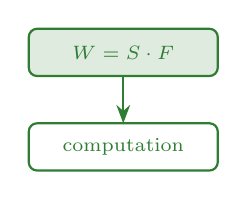
\begin{tikzpicture}[scale=0.6]
  \draw[grass,thick,rounded corners=3pt,fill=grass!15] (-2,2) rectangle (2,3);
  \node[font=\scriptsize,grass] at (0,2.5) {$W = S \cdot F$};
  \draw[grass,thick,-{Stealth}] (0,2) -- (0,1);
  \draw[grass,thick,rounded corners=3pt] (-2,0) rectangle (2,1);
  \node[font=\scriptsize,grass] at (0,0.5) {computation};
\end{tikzpicture}

\vspace{0.3em}
{\small Decomposes how the model \emph{computes}: $W_i = S_i \cdot F$.}

\vspace{0.2em}
{\small Guaranteed to be used --- every active factor is part of the computation.}
\end{column}
\end{columns}

\vspace{0.5em}
\centering
\fcolorbox{neutral}{bg}{\parbox{0.85\linewidth}{\centering\vspace{0.3em}
  {\small \textbf{The Grassmannian question applies to both:} whether the causal variable is linear determines whether SAE features, DAS subspaces, or factor-based directions can capture it.}
\vspace{0.3em}}}
\end{frame}


%% ============================================================
%% PART 5: IMPLICATIONS
%% ============================================================

\begin{frame}[plain]
\vfill
\begin{center}
  \setlength{\fboxrule}{2.5pt}%
  \fcolorbox{black}{white}{\parbox{0.7\textwidth}{\centering\vspace{0.8em}
    {\Large\bfseries Part 5}\hypertarget{part5}{}\\[0.5em]
    {\large Implications and practical advice}
  \vspace{0.8em}}}
\end{center}
\vfill
\end{frame}

\begin{frame}{In this section}
\begin{columns}[T]
\begin{column}{0.48\textwidth}
\textbf{\hyperlink{sec13}{15. Four-level hierarchy}}\\[0.2em]
{\small A hierarchy for causal validity: IIA alone is necessary but not sufficient. Faithfulness metrics and structural diagnostics provide increasingly strong evidence.}

\vspace{0.6em}
\textbf{\hyperlink{sec14}{16. Continuous metrics}}\\[0.2em]
{\small Binary IIA hides important differences. Continuous metrics (KL, logit diff) distinguish methods that all achieve IIA $\approx 1$.}
\end{column}
\begin{column}{0.48\textwidth}
\textbf{\hyperlink{sec15}{17. Practical advice}}\\[0.2em]
{\small Five concrete recommendations for causal abstraction practitioners: report faithfulness, use continuous metrics, validate nonlinear methods, test transfer.}

\vspace{0.6em}
\textbf{\hyperlink{sec16}{18. Conclusion}}\\[0.2em]
{\small The linearity assumption is testable. We provide both the diagnostics and the method to handle nonlinear variables.}
\end{column}
\end{columns}
\end{frame}

\hypertarget{sec13}{}
\section{13. Four-level hierarchy}

%% --- SLIDE: The hierarchy ---
\begin{frame}{A four-level hierarchy for causal validity}

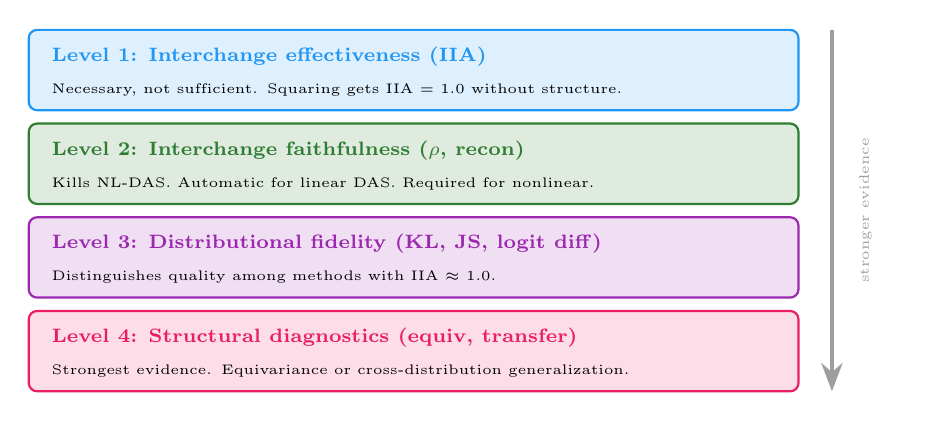
\begin{tikzpicture}[scale=0.85]
  % Level 1
  \fill[das!15,rounded corners=3pt] (-5.5,3.2) rectangle (6,4.4);
  \draw[das,thick,rounded corners=3pt] (-5.5,3.2) rectangle (6,4.4);
  \node[font=\scriptsize\bfseries,das,anchor=west] at (-5.3,4.0) {Level 1: Interchange effectiveness (IIA)};
  \node[font=\tiny,anchor=west,text width=10.8cm] at (-5.3,3.5) {Necessary, not sufficient. Squaring gets IIA = 1.0 without structure.};

  % Level 2
  \fill[grass!15,rounded corners=3pt] (-5.5,1.8) rectangle (6,3.0);
  \draw[grass,thick,rounded corners=3pt] (-5.5,1.8) rectangle (6,3.0);
  \node[font=\scriptsize\bfseries,grass,anchor=west] at (-5.3,2.6) {Level 2: Interchange faithfulness ($\rho$, recon)};
  \node[font=\tiny,anchor=west,text width=10.8cm] at (-5.3,2.1) {Kills NL-DAS. Automatic for linear DAS. Required for nonlinear.};

  % Level 3
  \fill[vae!15,rounded corners=3pt] (-5.5,0.4) rectangle (6,1.6);
  \draw[vae,thick,rounded corners=3pt] (-5.5,0.4) rectangle (6,1.6);
  \node[font=\scriptsize\bfseries,vae,anchor=west] at (-5.3,1.2) {Level 3: Distributional fidelity (KL, JS, logit diff)};
  \node[font=\tiny,anchor=west,text width=10.8cm] at (-5.3,0.7) {Distinguishes quality among methods with IIA $\approx$ 1.0.};

  % Level 4
  \fill[circle!15,rounded corners=3pt] (-5.5,-1.0) rectangle (6,0.2);
  \draw[circle,thick,rounded corners=3pt] (-5.5,-1.0) rectangle (6,0.2);
  \node[font=\scriptsize\bfseries,circle,anchor=west] at (-5.3,-0.2) {Level 4: Structural diagnostics (equiv, transfer)};
  \node[font=\tiny,anchor=west,text width=10.8cm] at (-5.3,-0.7) {Strongest evidence. Equivariance or cross-distribution generalization.};

  % Strength arrow
  \draw[neutral,ultra thick,-{Stealth}] (6.5,4.4) -- (6.5,-1.0);
  \node[font=\tiny,neutral,rotate=90] at (7.0,1.7) {stronger evidence};
\end{tikzpicture}

\vspace{0.5em}
{\small \textbf{Key asymmetry}: Linear DAS automatically passes Level 2 (orthogonal projection is faithful by construction) but may fail Level 1 on nonlinear variables. NL-DAS easily passes Level 1 but fails Level 2.}
\end{frame}

\hypertarget{sec14}{}
\section{14. Continuous metrics}

%% --- SLIDE: Binary vs continuous ---
\begin{frame}{Binary IIA hides important differences}

\begin{columns}[T]
\begin{column}{0.48\textwidth}
\centering
\textbf{Binary IIA}

\vspace{0.3em}
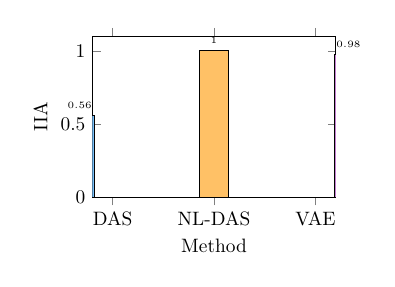
\begin{tikzpicture}[scale=0.7]
  \begin{axis}[
    width=6cm, height=4.5cm,
    ybar,
    bar width=15pt,
    xlabel={Method},
    ylabel={IIA},
    ymin=0, ymax=1.1,
    xtick={1,2,3},
    xticklabels={DAS,NL-DAS,VAE},
    ytick={0,0.5,1.0},
    nodes near coords,
    every node near coord/.append style={font=\tiny},
  ]
  \addplot[fill=das!60] coordinates {(1,0.556)};
  \addplot[fill=nldas!60] coordinates {(2,1.000)};
  \addplot[fill=vae!60] coordinates {(3,0.978)};
  \end{axis}
\end{tikzpicture}

{\small NL-DAS ``wins.'' But it is a lookup table.}
\end{column}
\begin{column}{0.48\textwidth}
\centering
\textbf{With faithfulness metrics}

\vspace{0.3em}
{\small\setlength{\tabcolsep}{2pt}
\begin{tabular}{lccc}
\toprule
& \textbf{DAS} & \textbf{NL-DAS} & \textbf{VAE} \\
\midrule
IIA & 0.556 & \textcolor{fail}{1.000} & \textcolor{pass}{0.978} \\
Diversity $\rho$ & 1.0 & \textcolor{fail}{$\approx 0$} & \textcolor{pass}{$\approx 1$} \\
Transfer & Yes & \textcolor{fail}{No} & \textcolor{pass}{Yes} \\
\bottomrule
\end{tabular}}

\vspace{0.5em}
{\small VAE wins genuinely. NL-DAS is disqualified by $\rho \approx 0$.}

\vspace{0.3em}
{\small DAS is honest but limited by linearity.}
\end{column}
\end{columns}
\end{frame}

\hypertarget{sec15}{}
\section{15. Practical advice}

%% --- SLIDE: Practical advice ---
\begin{frame}{Practical advice for causal abstraction}

\begin{enumerate}
  \item {\small \textbf{Never report IIA alone.} IIA = 1.0 is compatible with genuine structure, memorized lookup tables, and degenerate encoder-decoders. Always report at least one faithfulness metric.}

  \vspace{0.3em}
  \item {\small \textbf{Use continuous distributional metrics.} KL divergence and normalized logit difference distinguish among methods that all achieve IIA $\approx 1.0$. Binary IIA treats a 51\% shift the same as 99\%.}

  \vspace{0.3em}
  \item {\small \textbf{Be suspicious of unconstrained nonlinear featurizers.} Any encoder-decoder trained end-to-end on interchange loss without reconstruction constraints can learn a lookup table. The ELBO (or equivalent) is necessary.}

  \vspace{0.3em}
  \item {\small \textbf{Test cross-distribution generalization.} Evaluate on disjoint names, novel templates, or new task variants. A method that fails under distribution shift is exploiting surface regularities.}

  \vspace{0.3em}
  \item {\small \textbf{Consider nonlinear methods when DAS IIA is low.} Low IIA does not mean no causal variable --- it may mean DAS is searching the wrong function class. But validate with faithfulness metrics.}
\end{enumerate}
\end{frame}

%% --- SLIDE: Surprising cases ---
\begin{frame}{Surprising positive and negative cases}

\begin{columns}[T]
\begin{column}{0.48\textwidth}
\textbf{\textcolor{pass}{Surprising positives}}

\vspace{0.3em}
{\small \textbf{Cubic sum} ($a^3 + b^3$): perfect equivariance (100\%) despite cubing alone reaching only 50.9\%. The boundary is not ``group action vs.\ polynomial'' but whether the binary structure provides sufficient additive symmetry.}

\vspace{0.5em}
{\small \textbf{Max} ($\max(a,b)$): achieves 95.7\% equivariance despite not being a group action. It is piecewise equivariant: when the argmax is stable under shift, max behaves like a shifted identity.}
\end{column}
\begin{column}{0.48\textwidth}
\textbf{\textcolor{fail}{Surprising negatives}}

\vspace{0.3em}
{\small \textbf{Affine} ($2a + 3b + 5$): a \emph{linear} function that \emph{fails} to produce a Grassmannian variable! Under $a \mapsto a + g$, the output shifts by $2g$, not $g$. Equivariance requires the operation to be a group action, not merely linear.}

\vspace{0.5em}
{\small \textbf{Squaring}: achieves IIA = 1.0 by $k = 4$ without grokking. High IIA is the illusion; low equivariance (31.4\%) is the truth.}
\end{column}
\end{columns}
\end{frame}

\hypertarget{sec16}{}
\section{16. Conclusion}

%% --- SLIDE: Summary ---
\begin{frame}{Summary}

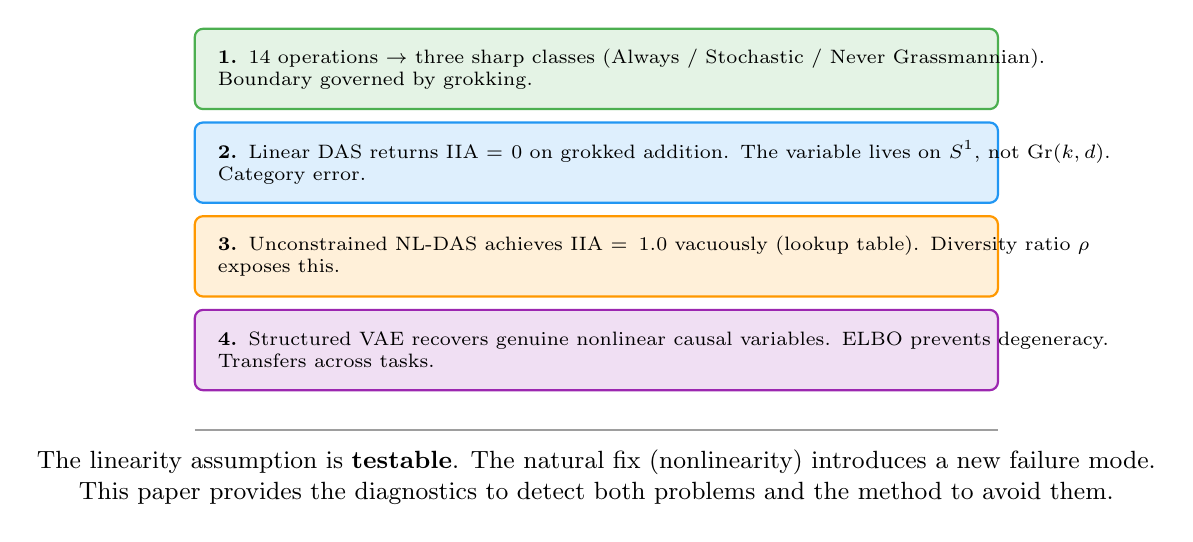
\begin{tikzpicture}[scale=0.85]
  % Finding 1
  \fill[always!15,rounded corners=3pt] (-5.5,3.0) rectangle (6.5,4.2);
  \draw[always,thick,rounded corners=3pt] (-5.5,3.0) rectangle (6.5,4.2);
  \node[font=\scriptsize,align=left,anchor=west,text width=11.5cm] at (-5.3,3.6) {\textbf{1.} 14 operations $\to$ three sharp classes (Always / Stochastic / Never Grassmannian). Boundary governed by grokking.};

  % Finding 2
  \fill[das!15,rounded corners=3pt] (-5.5,1.6) rectangle (6.5,2.8);
  \draw[das,thick,rounded corners=3pt] (-5.5,1.6) rectangle (6.5,2.8);
  \node[font=\scriptsize,align=left,anchor=west,text width=11.5cm] at (-5.3,2.2) {\textbf{2.} Linear DAS returns IIA $= 0$ on grokked addition. The variable lives on $S^1$, not $\Gr(k,d)$. Category error.};

  % Finding 3
  \fill[nldas!15,rounded corners=3pt] (-5.5,0.2) rectangle (6.5,1.4);
  \draw[nldas,thick,rounded corners=3pt] (-5.5,0.2) rectangle (6.5,1.4);
  \node[font=\scriptsize,align=left,anchor=west,text width=11.5cm] at (-5.3,0.8) {\textbf{3.} Unconstrained NL-DAS achieves IIA $= 1.0$ vacuously (lookup table). Diversity ratio $\rho$ exposes this.};

  % Finding 4
  \fill[vae!15,rounded corners=3pt] (-5.5,-1.2) rectangle (6.5,0.0);
  \draw[vae,thick,rounded corners=3pt] (-5.5,-1.2) rectangle (6.5,0.0);
  \node[font=\scriptsize,align=left,anchor=west,text width=11.5cm] at (-5.3,-0.6) {\textbf{4.} Structured VAE recovers genuine nonlinear causal variables. ELBO prevents degeneracy. Transfers across tasks.};

  % Bottom line
  \draw[neutral,thick] (-5.5,-1.8) -- (6.5,-1.8);
  \node[font=\small,align=center] at (0.5,-2.5) {The linearity assumption is \textbf{testable}. The natural fix (nonlinearity) introduces a new failure mode.\\This paper provides the diagnostics to detect both problems and the method to avoid them.};
\end{tikzpicture}
\end{frame}

%% --- SLIDE: The big picture ---
\begin{frame}{The big picture}

\begin{center}
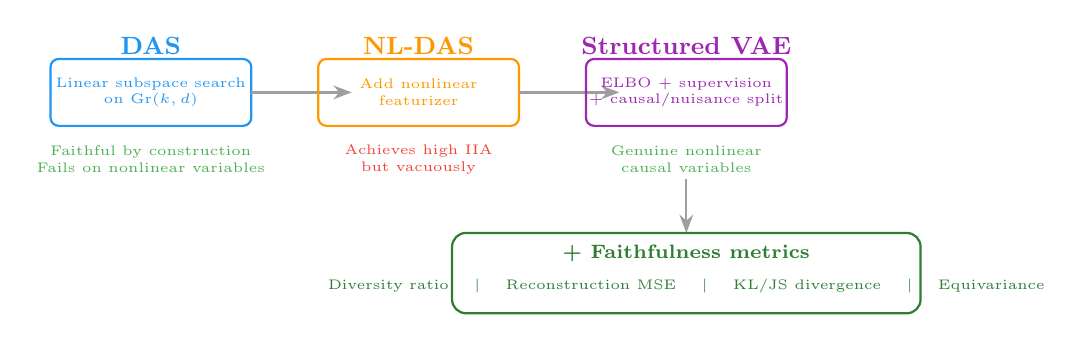
\begin{tikzpicture}[scale=0.85]
  % Timeline / flow
  \node[font=\small\bfseries,das] at (-4,3) {DAS};
  \draw[das,thick,rounded corners=3pt] (-5.5,1.8) rectangle (-2.5,2.8);
  \node[font=\tiny,das,align=center] at (-4,2.3) {Linear subspace search\\on $\Gr(k,d)$};
  \node[font=\tiny,pass,align=center] at (-4,1.3) {Faithful by construction\\Fails on nonlinear variables};

  \draw[neutral,thick,-{Stealth}] (-2.5,2.3) -- (-1,2.3);

  \node[font=\small\bfseries,nldas] at (0,3) {NL-DAS};
  \draw[nldas,thick,rounded corners=3pt] (-1.5,1.8) rectangle (1.5,2.8);
  \node[font=\tiny,nldas,align=center] at (0,2.3) {Add nonlinear\\featurizer};
  \node[font=\tiny,fail,align=center] at (0,1.3) {Achieves high IIA\\but vacuously};

  \draw[neutral,thick,-{Stealth}] (1.5,2.3) -- (3,2.3);

  \node[font=\small\bfseries,vae] at (4,3) {Structured VAE};
  \draw[vae,thick,rounded corners=3pt] (2.5,1.8) rectangle (5.5,2.8);
  \node[font=\tiny,vae,align=center] at (4,2.3) {ELBO + supervision\\+ causal/nuisance split};
  \node[font=\tiny,pass,align=center] at (4,1.3) {Genuine nonlinear\\causal variables};

  % Diagnostics below
  \draw[neutral,thick,-{Stealth}] (4,1.0) -- (4,0.2);
  \draw[grass,thick,rounded corners=5pt] (0.5,-1.0) rectangle (7.5,0.2);
  \node[font=\scriptsize\bfseries,grass] at (4,-0.1) {+ Faithfulness metrics};
  \node[font=\tiny,grass,align=center] at (4,-0.6) {Diversity ratio \quad $|$ \quad Reconstruction MSE \quad $|$ \quad KL/JS divergence \quad $|$ \quad Equivariance};
\end{tikzpicture}
\end{center}

\vspace{0.5em}
\centering
{\small Every causal abstraction claim should be evaluated with the \textbf{four-level hierarchy}.\\IIA is necessary but never sufficient.}
\end{frame}

%% --- SLIDE: Thank you ---
\begin{frame}[plain]
\vfill
\begin{center}
{\Large\bfseries Thank you}

\vspace{1em}
{\small Code and experiments:\\
\texttt{github.com/elliottower/grokking-causal-geometry}}

\vspace{0.5em}
{\small Elliot Tower \quad $\cdot$ \quad Ivan Vegner \quad $\cdot$ \quad N.\ Siddharth \quad $\cdot$ \quad Alex Doumas}

\vspace{1em}
{\small \textcolor{neutral}{Draft paper: \emph{When Does Linear Causal Abstraction Work?\\Mapping the Boundary on the Grassmannian}}}
\end{center}
\vfill
\end{frame}

\end{document}
